\chapter[Columnar clusters in the human motion complex reflect consciously perceived motion axis]{Columnar clusters\\ in the human motion complex\\ reflect consciously perceived\\ motion axis}
\chaptermark{Columnar clusters in hMT+ reflect conscious motion axis}
\papercitetwo

\clearpage{\thispagestyle{empty}\cleardoublepage}

\section{Abstract}
The specific contents of human consciousness rely on the activity of specialized neurons in cerebral cortex. We hypothesized that the conscious experience of a specific visual motion axis is reflected in response amplitudes of direction-selective clusters in the human motion complex. Using sub-millimeter functional magnetic resonance imaging at ultra-high field (7 Tesla) we identified fine-grained clusters that were tuned to either horizontal or vertical motion presented in an unambiguous motion display. We then recorded their responses while human observers reported the perceived axis of motion for an ambiguous apparent motion display. Although retinal stimulation remained constant, subjects reported recurring changes between horizontal and vertical motion percepts every 7 to 13 seconds. We found that these perceptual states were dissociatively reflected in the response amplitudes of the identified horizontal and vertical clusters. We also found that responses to unambiguous motion were organized in a columnar fashion such that motion preferences were stable in the direction of cortical depth and changed when moving along the cortical surface. We suggest that activity in these specialized clusters is involved in tracking the distinct conscious experience of a particular motion axis.

% \papercitation{Schneider2019}{Printed}

\section{Introduction}
An important goal of neuroscience research is to dissociate neural signals pertaining to conscious perception from those related to sensory stimulation \parencite{Logothetis1989, Rees2007}. Experimentally, this can be achieved by exposing observers to multistable stimuli, i.e. stimuli that lead to changes in perception despite unchanging stimulation of the senses \parencite{Leopold1999, Sterzer2009, Brascamp2018}. For example, the bistable motion quartet (Figure ~\ref{fig:paradigm}A, upper panel) yields conscious perception of either horizontal or vertical motion \parencite{Ramachandran1985}. The perceived axis of motion switches every few seconds although the retinal stimulation remains constant. Only those neurons that modulate their activity with the perceived axis of motion should be considered content-specific neural correlates of consciousness (NCC) \parencite{Metzinger2000, Koch2016}.

\begin{figure}[htb!]
\centering
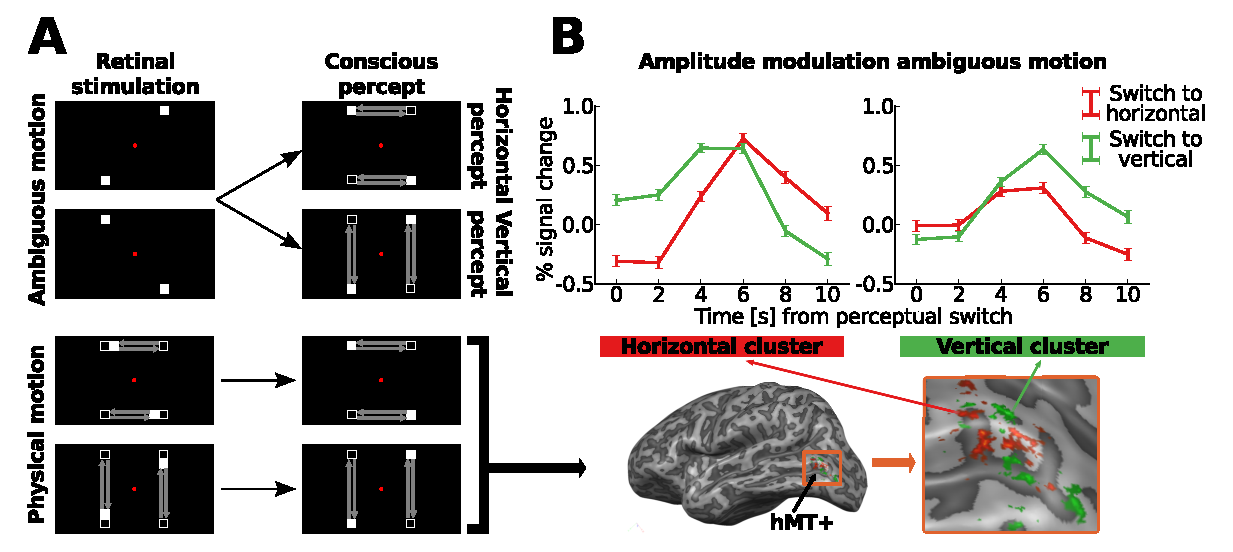
\includegraphics[width=\textwidth]{figures/chapter_03/fig1.eps}
% {\bfseries Experimental paradigm and event-related averages.}
\caption{Experimental paradigm and event-related averages. \textbf{(A)} Overview of experimental paradigm. During the “ambiguous motion” experiment (top), the bistable motion quartet was presented. Presenting two opposed square pairs in temporal alternation gives rise to the conscious percept of either horizontal or vertical apparent motion. While the percept switches about every 10 seconds, the retinal stimulation remains constant throughout the experiment. During the “physical motion” experiment (bottom), squares moved physically along the horizontal or vertical motion paths that were previously only perceived during the ambiguous motion experiment. Physical motion led to unambiguous horizontal or vertical percepts. \textbf{(B)} The physical motion stimulus elicited responses in area hMT+, here displayed on the inflated, left hemisphere of a representative subject (bottom). These responses distinguished horizontal (red) and vertical (green) motion clusters. We studied responses in these clusters to the ambiguous motion experiment (top): Lines show event-related weighted averages across all subjects. Percent signal change is displayed during horizontal (red lines) and vertical (green lines) perceptual periods, as indicated by the subjects via button presses. At time point 0s subjects reported a perceptual switch specifying whether they now perceived horizontal or vertical motion. Error bars represent the uncertainty of the mean.}
\label{fig:paradigm}
\end{figure}

Multistable paradigms have revealed strong correlations between the experience of visual motion and responses in both the monkey and human middle temporal visual complex (MT+ and hMT+) \parencite{Leopold1999, Rees2007, Sterzer2009}. When macaque monkeys are trained to signal their conscious percept during binocular rivalry, about 40 percent of MT+ neurons sampled during electro-physiological recordings modulate their spiking with the perceived direction of motion \parencite{Logothetis1989, Leopold1999}. Equally, during the presentation of bistable figures, neurons in MT \parencite{Dodd2001}, medial superior temporal (MST) and parietal cortex \parencite{Williams2003} all show activity reflecting the consciously perceived direction of motion. Monkey areas MT and MST are also spatially organized into columns and clusters of neurons that are each tuned to a particular motion direction \parencite{Albright1984, Salzman1990, Britten1998}. Yet it is unclear whether the NCC for motion direction is localized to these structures.

In humans, the functional magnetic resonance (fMRI) response in area hMT+ as a whole reflects conscious motion perception. Responses are increased for apparent as opposed to flicker motion \parencite{Muckli2002} and with reversals in perceived motion direction \parencite{Sterzer2002}. When subjects indicate that they perceive horizontal component motion, the hMT+ amplitude is higher than for vertical pattern motion \parencite{Castelo-Branco2002}. Furthermore, attended motion directions can be decoded from area hMT+ \parencite{Kamitani2006} and hMT+ signals predict perceptual states of clockwise or counterclockwise motion during ambiguous structure-from-motion \parencite{Brouwer2007}. Like monkey MT, hMT appears to be organized into columnar clusters \parencite{Zimmermann2011}. To reveal this organization, however, advances in MRI technology \parencite{Ugurbil2003} and analysis strategies \parencite{Kemper2017,Polimeni2017} were necessary that allow measuring fMRI responses at sub-millimeter spatial resolution. Until now fMRI studies on conscious motion perception have used relatively low resolutions (18 - 54 mm3) and could not investigate whether responses in distinct clusters within hMT+ relate to experience of a specific motion axis.

We recorded sub-millimeter fMRI responses from area hMT+ while humans viewed the bistable motion quartet stimulus and reported the perceived axis of motion via button presses. We hypothesized that (i) hMT+, like monkey MT+, has distinct functional subunits that each modulate with the perceptual state of a particular motion axis and (ii) that these units display a spatial organization into columnar clusters.

\section{Methods}
\subsection{Participants}
Nine healthy participants with corrected- to- normal vision were recruited for the study. All participants were students or employees of Maastricht University and recruitment was limited to participants who were MRI compatible and had been in an MRI scanner at least once before to ensure high subject compliance. Additionally, all participants were experienced in fixation tasks. Four participants (S2, S4, S5, S6) were excluded from further data analysis (S2 did not show up for the second scanning session; S4 performed the task inappropriately during scanning, pressing buttons to indicate perceptual switches every 200 - 400 ms; S5 showed excessive head movement and S6 did not perceive stable states of horizontal and vertical apparent motion during the training session). Hence, five participants (3 females, 23-28 years old) were analyzed. All participants gave informed, written consent to participate in the experiment. The study was approved by the research ethics committee of the Faculty of Psychology and Neuroscience of Maastricht University.

\subsection{Experimental design and stimuli}
Visual stimuli were created and presented using the open-source application PsychoPy (version 1.82.01) \parencite{Peirce2007,Peirce2008}. Stimuli were projected on a frosted screen at the head end of the scanner (using Panasonic projector PT-EZ570; Newark, NJ, USA; resolution 1920 x 1200; nominal refresh rate: 60 Hz). Subjects viewed the screen via a tilted mirror attached to the head coil. Button responses were registered using an MR compatible button box (Current Designs, 8-button response device, HHSC-2 × 4-C; Philadelphia, USA). All scripts used for stimulus presentation are available as \href{https://github.com/MSchnei/motion_quartet_scripts}{GitHub} and \href{https://zenodo.org/record/1489246}{zenodo repository}.

For every subject we collected 3 runs to localize area hMT+ (240 volumes, 12 repetitions per condition per run), 5-6 runs of the ambiguous motion experiment (300 volumes, $ 22.30 \pm 1.14$ (mean $\pm$ standard deviation) repetitions per condition per run) and 5-6 runs of the physical motion experiment (300 volumes, 24 repetitions per condition per run). These runs were acquired across two different scanning sessions on separate days. Additionally, we performed three control experiments to exclude the possibility that observed differences between horizontal and vertical conditions were driven by retinotopic differences: For two subjects (S1 and S3), we acquired 3 runs (204 volumes, 6 repetitions per condition per run) to estimate axis-of-motion tuning curves (control experiment I) which were recorded during the first scanning session of the motion quartet experiments. Three subjects (S1, S3, S9) were recruited for an additional, third scanning session and we acquired 5-8 runs (222 volumes, 12 repetitions per condition per run) to map out responses to retinotopically identical horizontal and vertical motion conditions (control experiment II). Finally, for two subjects (S3 and S7) we organized a fourth scanning session to obtain 6 runs (172 volumes per run, in total 27 repetitions per aperture position) of data that allowed us to estimate population receptive field (pRF) parameters (control experiment III).

\subsubsection{hmt+ localizer}
Area hMT+ was localized using standard moving and static dot stimuli \parencite{Huk2002, Amano2009, Emmerling2016} presented in a circular aperture (10° of visual angle in diameter) that was either centered or displaced by 5° of visual angle to the left or right. All dots (200 dots; 0.2° in diameter; white on black background) moved at 8° per second and were either expanding or dilating, alternating direction every second. Every dot had a limited life time of 167 ms (10 frames) and was reborn at a randomized location within the aperture. 4s periods of moving dots were followed by periods of static dots (randomized duration: either 6s, 8s or 10s). The aperture position for static dots always matched the preceding aperture position for moving dots. Participants were asked to fixate on a centrally presented dot throughout the entire experimental run. The fixation dot consisted of a red circle surrounded by a yellow annulus \parencite{Marquardt2018}. The fixation dot occasionally (20 targets per run) changed color from red to yellow for 0.3 s and participants indicated a color change by pressing a button.

\subsubsection{Ambiguous and physical motion experiment}
Participants were presented with two different motion quartet stimuli - an "ambiguous" and a disambiguated or "physical" version. In the ambiguous version (Experiment 1) we used the apparent motion quartet \parencite{Ramachandran1985} (see upper panel Figure ~\ref{fig:paradigm}). The quartet is composed of four blinking squares (each 1° x 1° visual angle) in a rectangular configuration. Crucially, at any time point, only two squares at diagonally opposite corners are shown. A pair of squares was presented for 150 ms (9 frames) followed by an inter-stimulus interval of 67 ms (4 frames). Such a presentation frequency of 2.3 Hz was shown to lead to strong perception of apparent motion \parencite{Finlay1987}.

In the physical version (Experiment 2) squares moved unambiguously either horizontally or vertically. This was achieved by physically moving white squares along the motion paths that were previously only perceived in Experiment 1 (see lower panel Figure ~\ref{fig:paradigm}A). Square positions were updated according to a harmonious oscillation, where the square location was updated as the sine of time \parencite{Muckli2005}. Stimulus parameters in Experiment 2 were matched to those in Experiment 1: Square size remained 1° x 1° of visual angle. Outermost horizontal and vertical points of the physical motion trajectory were equivalent to square positions in Experiment 1 (individually adjusted for every subject during a training session, see below). Duration of a movement cycle either along the horizontal (left to right to left) or vertical trajectories (top to bottom to top) was 433 ms (26 frames), which matched the presentation frequency in Experiment 1.

The ambiguous motion quartet was shown during periods of 40s, which were interleaved with 16s baseline periods. A flicker motion quartet in which all four squares were shown synchronously served as the baseline. This local flicker stimulus did not induce apparent motion but still had the same stimulus energy as the regular motion quartet. Participants were instructed to fixate a red dot in the center of the screen throughout the experiment and to indicate the perceived axis of motion (vertical or horizontal) by button responses. The mapping of perceived motion axis to buttons (whether button "1" or button "2" was used to indicate horizontal or vertical motion) was counterbalanced across the two scanning sessions.

The physical motion stimulus was equally shown during periods of 40 s in total. However, this time the motion axis was unambiguous and alternated every 10 s between horizontal and vertical motion. During the 16 s baseline period, participants again viewed the flicker motion quartet. They fixated the central red dot and indicated the perceived axis of motion by button responses. This was done although the motion axis was clearly determined by the stimulus, in order to engage participants in a task and to keep the task constant across Experiments 1 and 2.

\subsubsection{Control experiment I: axis-of-motion tuning}
In order to determine the axis-of-motion tuning of voxels, we presented moving and static dot stimuli in a central aperture (aperture diameter 10° visual angle; 200 dots; 0.2° in diameter; white on black background) such that the aperture field covered the real and perceived motion trajectories in Experiments 1 and 2. There were four different conditions, each corresponding to one of four axes of motion (0°-180°, 45°-225°, 90°-270°, 135°-315°; thus including the vertical and horizontal motion axes occupied in Experiments 1 and 2). 6s periods of moving dots were interleaved with static rest periods that lasted 8s, 10s or 12s. The order of conditions was randomized. During axis-of-motion blocks the direction of dots alternated every second; e.g. during the 0°-180° condition leftward motion alternated with rightward motion. Dots were moving at a speed of 8° of visual angle per second. Participants performed the same fixation task as described for the hMT+ localizer.

\subsubsection{Control experiment II: moving dot pattern}
In order to determine the tuning of voxels to motion either along the horizontal or vertical axis, we repeated control experiment I with two modifications. First, instead of four there were only two conditions, showing dots moving either along the horizontal (0°-180°) or vertical (90°-270°) motion axis. Second, visibility of the dots was restricted to a square annulus aperture. Shape and location of the aperture were defined as to reveal positions in visual space that had been occupied during the motion quartet experiments (simultaneously the locations of both horizontal and vertical motion trajectories as well as the four inducer squares, see Figure ~\ref{fig:figI_motionTng}C). Importantly, this resulted in the horizontal and vertical motion conditions being retinotopically identical and only differing with regard to the motion axis of the dots revealed by the aperture. Area hMT+, unlike areas V1-V3, does not display an aperture bias resulting in higher responses at retinotopic locations where moving dots enter the stimulus aperture, making this experimental set-up suitable to study the question of interest here \parencite{Wang2014}. The aperture was adjusted for every control subject to match subject-specific vertical distances (Table ~\ref{tab:distances}). Other parameters were identical to those reported for control experiment I.

\subsubsection{Control experiment III: population receptive field mapping}
The pRF mapping stimuli consisted of apertures that took the shape of semi rings and were presented at systematically varied positions. A single semi ring aperture had a radial extent of 3° of visual angle and subtended 180 angular degrees. Apertures were presented at four orientations (horizontal, vertical and the two diagonal orientations in-between) and at four eccentricity levels (centered on eccentricities of 1.5°, 4.5°, 7.5°, and 10.5° of visual angle). Apertures at the innermost eccentricity level (1.5°) consisted of semi circles, not semi rings. All apertures were limited to a circular region of the display, 24° of visual angle in diameter, and presented against a mean luminance gray background.

The carrier pattern of the mapping stimuli consisted of a random texture pattern as described by \cite{Kolster2010} and was presented at 98.2\% Michelson contrast (which was the highest possible contrast in the scanner environment). Aperture positions were updated with every TR (3s) and in a pseudo-random fashion such that two subsequent apertures never overlapped retinotopically. Every functional run started and ended with 15 s blank screen. To aid the estimation of large pRFs, 18 x 3s periods of blank screen were inserted throughout the functional run \parencite{Amano2009}.

Participants performed the same fixation task as described for the hMT+ localizer. To facilitate central fixation, an extended grid of thin lines was presented throughout the experimental run \parencite{Tyler2005}. The grid consisted of two diagonal, orthogonal lines crossing behind the fixation dot as well as circles with radii of 1, 2.5, 5, 10 and 15 degrees of visual angle centered on the fixation dot.

\subsubsection{Pre-scan training session}
With central fixation, observers of the ambiguous motion quartet more frequently perceive vertical than horizontal motion \parencite{Glaser1991}. This is thought to reflect the cost of inter-hemispheric processing, which is necessary for horizontal but not for vertical motion \parencite{Glaser1991, Gen2011}. To ensure that the motion quartet stimulus was bistable, i.e. that horizontal and vertical perceptual intervals were approximately equal in length, we scheduled a 20-30 minutes training session for every participant before the first scanning session. During this training session, we kept the horizontal distance between squares of the motion quartet constant (3° visual angle from square center to central fixation point), while we adjusted the vertical distance of the squares for every subject to obtain a bistable stimulus display. Table ~\ref{tab:distances} shows the resulting subject-specific vertical distances. The ratio of vertical to horizontal distances was between 1.26 and 1.30 for all subjects, which is in agreement with previously reported ratios for motion quartet stimuli to achieve equal frequencies \parencite{Glaser1991}. Once the vertical distance had been calibrated for a subject, it was kept constant across Experiment 1 and 2 and the two scanning sessions.

\subsection{Mri acquisition}
Data acquisition was performed on a whole-body Magnetom scanner (nominal field strength 7 Tesla, Siemens Medical Systems, Erlangen, Germany) at the Maastricht Brain Imaging center, The Netherlands. All images were acquired using a 32-channel head-coil (NovaMedical Inc.; Wilmington, MA, USA).

\subsubsection{hmt+ localizer}
To aid the positioning of the sub-millimeter slab for Experiments 1-2 and to determine our region of interest, we acquired one hMT+ localizer scan in the first session and two hMT+ localizer scans in the second session. We used a 2D gradient echo (GE) echo planar imaging (EPI) sequence (1.6 mm isotropic nominal resolution; TE/TR = 18/2000 ms; in-plane field of view (FoV) 150×150 mm; matrix size 94 x 94; 28 slices; nominal flip angle (FA) = 69°; echo spacing = 0.71 ms; GRAPPA factor = 2, partial Fourier = 7/8; phase encoding direction head - foot). We ensured that the area of acquisition had bilateral coverage of the posterior inferior temporal sulci, where we expected the hMT+ areas. Before acquisition of the first functional run, we collected 10 volumes for distortion correction - 5 volumes with the settings specified above and 5 more volumes with identical settings but opposite phase encoding (foot - head).

\subsubsection{Ambiguous and physical motion experiment}
For the sub-millimeter measurements, we used a 2D GE EPI sequence (TE/TR = 25.6/2000 ms; in-plane FoV 148×148 mm; matrix size 186 x 186; slices = 28; nominal FA = 69°; echo spacing = 1.05 ms; GRAPPA factor = 3, partial Fourier = 6/8; phase encoding direction head - foot), yielding a nominal resolution of 0.8 mm isotropic \parencite{Moeller2010, Setsompop2012}. Placement of the small functional slab was guided by online analysis of the hMT+ localizer data recorded immediately at the beginning of the first session. This allowed us to ensure bilateral coverage of area hMT+ for every subject. In the second scanning session, the slab was placed using Siemens auto-align functionality and manual corrections. Before acquisition of the first functional run, we collected 10 volumes for distortion correction (5 volumes with opposite phase encoding: foot - head). During acquisition, runs for the ambiguous and physical motion experiments were interleaved.

\subsubsection{Control experiments}
The acquisition parameters for control experiments I and II were identical to those reported for the motion quartet experiments. For the pRF mapping, we used the same 2D GE EPI sequence as in the motion quartet experiments with slightly adjusted parameters to obtain a larger field of view (in particular, multi band factor = 2; TE/TR = 23.2/3000 ms; in-plane FoV 140×140 mm; matrix size 176 x 176; slices = 82; nominal resolution = 0.8; nominal FA = 82°; echo spacing = 1.04 ms; GRAPPA factor = 3; partial Fourier = 6/8; phase encoding direction head - foot) \parencite{Moeller2010, Setsompop2012, Feinberg2010}.

\subsubsection{Anatomical scans}
For visualization of the functional results, we acquired scans with structural information in the first scanning session. At high magnetic fields, MR images exhibit high signal intensity variations that result from heterogeneous RF coil profiles \parencite{Moortele2009}. We therefore acquired both T1w images and PDw images using a magnetization-prepared 3D rapid gradient-echo (3D MPRAGE) sequence (TR: 3100 ms (T1w) or 1440 ms (PDw), voxel size = 0.6 mm isotropic, FOV = 230 x 230 mm2, matrix = 384 x 384, slices = 256, TE = 2.52 ms, FA = 5°). Acquisition time was reduced by using 3× GRAPPA parallel imaging and 6/8 Partial Fourier in phase encoding direction (acquisition time (TA): 8 min 49 s (T1w) and 4 min 6 s (PDw)).

\subsection{Behavioral data analysis}
For every subject we calculated the mean length of horizontal and vertical perceptual periods during the ambiguous motion experiment. To test for differences between horizontal and vertical periods, we conducted an independent-samples t-test for every subject (p\textless.05, two-sided). We also calculated the mean, standard deviation and range across subjects for the two types of perceptual periods.

\subsection{Structural data analysis and segmentation}
Structural images were processed using advanced segmentation tools in BrainVoyager 20.0 (Brain Innovation, Maastricht, The Netherlands), SPM's bias correction \parencite{Ashburner2005}, ITK-SNAP \parencite{py06nimg}, FSL BET \parencite{Smith2002}, morphological operations \parencite{scipy2001} and Segmentator \parencite{Gulban2018a}. Where not specified otherwise, default settings were used. Since the processing included many different steps and programs, a diagram of the input/output relationships for all processing steps is provided in Figure ~\ref{fig:figAB_proc}A. We first registered the PDw image for every subject to their T1w image, using ITK-SNAP's automatic co-registration tools. In order to reduce the B1 bias field, we divided the T1w image by the PDw image and obtained a ratio image \parencite{Moortele2009}. The ratio image was brain-masked with a masked obtained by inputting the co-registered PDw image to FSL BET. We then used SPM's anatomical bias correction to further reduce inhomogeneities in the ratio image.

The resulting image was input to BrainVoyager's advanced segmentation routine to obtain a white matter (WM) definition. This initial WM image was inspected and manually polished in ITK-SNAP using the adaptive paint brush mode in combination with a graphics tablet (Intuos Art; Wacom Co. Ltd; Kazo, Saitama, Japan). Special emphasis was placed on corrections in the region of interest (bilateral hMT+). In two additional steps, using the round paint brush mode, the parts of the cerebellum and sagittal sinus that were falsely included in the WM definition were removed and brain stem structures and ventricles were masked.

The thus polished WM definition and ratio image were input to BrainVoyager's advanced segmentation routine to obtain a gray matter (GM) definition. This GM definition tended to be too inclusive, containing dura mater and blood vessels. For this reason, we masked the ratio image with the WM and GM definitions and input the resulting image to Segmentator. This allowed us to further exclude non-brain voxels from the GM definition based on their 2D histogram profile along the dimensions of image intensity and gradient magnitude. The thus improved GM definition was inspected and further polished manually in ITK-SNAP using the round paint brush mode. For later mesh visualization, the WM-GM segmentation images were separated in two hemispheres using ITK-SNAP's scalpel tool. Remaining topological errors were corrected using the bridge removal option in BrainVoyager \parencite{Kriegeskorte2001} and manual correction. Note that all segmentation steps were performed at the original resolution of the anatomical images (0.6 mm isotropic).

\subsection{Functional data - preparation}
Functional data were processed using BrainVoyager 20.0, SPM 12 \parencite{Friston2006}, FSL 5.0 \parencite{Jenkinson2012} as well as custom code in Python 2.7 \parencite{numpy2011, scipy2001, matplotlib2007} and in Matlab R2014a (The Mathworks Inc.; Natick, MA, USA). Where not specified otherwise, default settings were used. All functional pre-processing steps were scripted and scripts are available as a \href{https://github.com/MSchnei/motion_quartet_scripts}{GitHub} and \href{https://zenodo.org/record/1489246}{zenodo repository}. Figure ~\ref{fig:figAB_proc}B provides an overview of all functional pre-processing steps. 

\subsubsection{Pre-processing steps}
Pre-processing for all sub-millimeter images was performed in the following order: slice scan time correction (BrainVoyager), motion-correction (SPM 12), linear trend removal and high-pass filtering (5 cycles) using a general linear model (GLM) Fourier basis set (BrainVoyager) and distortion correction (FSL topup). For motion and distortion correction, we deviated from default settings. Functional images from the first session were motion-corrected using SPM 12 in three steps. First, the first image of each run was realigned to the first image of the first run. Second, the images within each run were aligned to the first image of the run. Third, to avoid local minima, after these first two steps, a mean of all images was calculated and images were realigned to this mean. Motion correction was limited to voxels inside the brain based on an intensity-thresholded and manually corrected brain mask of the functional images. Note that the results of the three steps were combined into a single transformation that was applied to functional images to minimize interpolation artefacts. Functional images from the second scanning session were motion-corrected in a similar vein, with the difference that the first functional image of the second session served as reference image in the first correction step. Steps 2 and 3 were identical. For details on the alignment across scanning sessions, please see below. EPI distortions of the functional images were corrected using FSL topup \parencite{Andersson2003, Smith2004}. The pairs of opposite phase encoding images acquired at the beginning of the first session were input to topup to estimate the susceptibility-induced off-resonance field. The estimated field was then used to correct the distortions for all functional images of the first and second scanning session. For the MT+ localizer images, pre-processing steps included slice scan time correction, motion-correction, linear trend removal combined with high-pass filtering (all performed in BrainVoyager) and distortion correction (FSL topup). In addition to the pre-processing steps described above, we applied Gaussian spatial smoothing (smoothing kernel = 0.8 mm) to the pRF mapping data, reflecting the prior assumption that pRF parameters vary smoothly over space.

\subsubsection{Registration to functional images}
All statistical analyses were conducted in the space of the sub-millimeter functional images in the first scanning session (hereafter called "voxel space"). To this end, the pre-processed anatomical T1w-divided-PDw ratio image was registered to voxel space by exploiting the scanner’s positional information and fine-tuning co-registration with boundary-based registration \parencite{Greve2009} as implemented in BrainVoyager. The result was visually inspected for each subject by overlaying functional and anatomical images (anatomical images were displayed with inverted image intensities for better visualization). Co-registration and down-sampling of the anatomical image were performed in one step.

In order to register the high-resolution segmentation images (0.6 mm isotropic) to lower-resolution voxel space (0.8 mm isotropic) we proceeded as follows. Problematically, simply transforming an image with only two segmentation values (for WM and GM) results in interpolation artefacts and how to bin the resulting distribution of values to regain only two segmentation values is not obvious. For that reason, we performed a surface reconstruction of both the inner and outer GM border in BrainVoyager. This resulted in two different surface meshes to which we applied the established transformation from anatomical images to voxel space. Transformed meshes were smoothed, using advanced mesh smoothing tools (restricting vertex displacement to 0.5). Importantly, the advanced mesh smoothing is restricted to high-frequencies and leaves low-frequency changes such as cortical folds intact. Smoothed meshes were projected back into volume space and area filling tools were used to regain a segmentation image with only two values. We inspected the resulting WM-GM segmentation images in voxel space separately for every subject and found this procedure to preserve important features of the segmentation and to minimize the re-introduction of topological errors (see Figure ~\ref{fig:figC_segmQual}A). Re-introduced errors were manually corrected using itksnap. This was limited to 20-30 mislabeled voxels in our region of interest.

hMT+ localizer functional images acquired in the second session were first registered to the anatomical images in the first session based on the scanner’s positional information, manual corrections, and boundary-based registration \parencite{Greve2009} for fine-tuning. Subsequently, the already established transformation from anatomical images to voxel space was used. MT+ localizer functional images were up-sampled from 1.6 mm isotropic to 0.8 mm isotropic using nearest-neighbor interpolation. All transformations were combined and applied in a single step to avoid unnecessary interpolation.

To align the sub-millimeter functional images acquired in the second scanning session (and in the control experiments) to voxel space, we chose a more complex procedure than for the hMT+ localizer functional images. This was because we found EPI distortions to differ across scanning sessions for sub-millimeter functional images and simply co-registering both (distortion-corrected) functional sessions to the anatomy did not meet our quality demands for sub-millimeter analyses. For that reason, we calculated a mean image across time, separately for every scanning session (before EPI-distortion correction). We then ran an initial affine registration between the mean image of the first session and each of the mean images of the other sessions using FSL FLIRT \parencite{Jenkinson2001, Jenkinson2002} with 12 degrees of freedom (dof) and, since we noticed residual distortion differences, a subsequent non-linear registration using FSL FNIRT \parencite{Andersson2007}. The resulting linear and non-linear transformations were combined into a single transform, which was applied to all sub-millimeter images recorded outside the first scanning session. We visually inspected the quality of the resulting alignment between the first run in the first session and all runs in the other sessions. Only then EPI distortion correction was applied to the transformed images, using the off-resonance field estimated in session 1. We applied a mask to all images, excluding voxels that had a mean intensity value below 12 in at least one of the sessions. This excluded voxels at the fringes of the slabs (due to minimal differences in slab placement across the two sessions) and we verified that voxels in our region of interest (ROI) were not affected.

\subsubsection{Roi definitions}
In order to define our ROI (bilateral hMT+), we calculated a voxel-wise general linear model (GLM) on a single-subject level for the hMT+ localizer data. The GLM was corrected for temporal auto-correlation (AR2). The model contained a separate predictor for the three stimulus conditions (moving dots in the left, central and right aperture). We selected voxels that showed a significant response to the central condition (using a threshold (q) corrected for multiple comparisons using false discovery rate; q(FDR)\textless.05; S1: t(474)\textgreater3.00; S3: t(474)\textgreater2.80; S7: t(474)\textgreater2.68; S8: t(474)\textgreater2.81; S9: t(474)\textgreater2.75). For each hemisphere, we projected this selection of voxels onto the inflated surface reconstructed along the middle of gray matter (for every vertex, the maximum statistical value in a range from -2mm to +2mm from the middle of gray matter was displayed). This allowed us to delineate area hMT+ on each hemisphere by manual drawing. Although drawing introduced a component of subjective judgment, the degree of subjectivity was minimal given that the areas were clearly outlined by significant responses (for an example, see Figure ~\ref{fig:figD_roiSel}). Significant responses needed to be located at the posterior/dorsal limb of the inferior temporal sulcus to be included in the ROI, in keeping with previous empirical work reporting the location of area hMT+ \parencite{Dumoulin2000, Huk2002, Kolster2010}. Figure ~\ref{fig:figE_MtLoc} shows the resulting definitions on the surface for left and right hemispheres. The surface patches were projected back into volume space (from -2mm to +2mm from the middle of gray matter) and restricted to GM. Delineations on the left and right hemisphere were grouped together to constitute a single ROI per subject. Table ~\ref{tab:rois} lists the number of voxels included in the ROIs as well as the estimated areas of left and right hMT+ on the surface. In summary, three criteria thus determined the selection of voxels for our ROI: (1) significant responses to central condition of independent hMT+ localizer data, (2) anatomical position at the posterior/dorsal limb of ITS, (3) voxels needed to be in GM.

\subsection{Functional data - statistical analyses}
To form single-subject event-related averages for the ambiguous motion experiment (Experiment 1), we converted every voxel's response to percent signal change where the mean of the respective run time series served as baseline. Separately for each cluster, signals were first averaged across voxels and then grouped by time point during horizontal and vertical perceptual periods. This resulted in event-related averages from time point 0s (subjects indicated a perceptual switch) until 10s later (average length of a perceptual period), in steps of 2s (our TR). In total, there were four event-related averages per subject (2 clusters x 2 perceptual periods). Event-related averages for the physical motion experiment (Experiment 2) were created in a similar fashion, with the following modification. To avoid circularity, we used a leave-one-run-out cross-validation scheme where all runs but one were used to assign voxels to either the horizontal or vertical cluster and responses from the left-out run were averaged across the cross-validation folds.

To obtain event-related averages across all subjects and to take differences in number of perceptual periods per subject into account, we calculated a weighted mean per time point \parencite{Cohen1998}, according to 
\begin{equation}
\overline{x}_{tp} = \frac{\sum\limits_{i=1}^n \frac{1}{\sigma_i^2} x_i}{\sum\limits_{i=1}^n \frac{1}{\sigma_i^2}}
\end{equation}

where $n$ is the number of subjects, $x_i$ is the mean per subject per time point, and $\sigma_i$ is the standard deviation across perceptual periods per subject per time point. Uncertainty in $\overline{x}_{tp}$ for display of the error bars was calculated using error propagation \parencite{Cohen1998} as
\begin{equation}
\sigma_{tp} = 1 / \sqrt{\sum\limits_{i=1}^n \frac{1}{\sigma_i^2}}
\end{equation}

To test for statistical significance of the amplitude modulations observed during the ambiguous motion experiment, we computed a general linear model (GLM) containing predictors for horizontal and vertical motion and calculated t-values for the contrast horizontal \textgreater vertical in horizontal clusters and for the contrast vertical \textgreater horizontal in the vertical cluster (empirical t-values). We then obtained a null distribution of t-values by randomly permuting condition labels and rerunning the GLM analysis (1000-fold permutation testing). If the empirical t-value was above the 97.5th percentile of the null distribution, the modulation for a cluster was declared significant. This amounts to a two-sided hypothesis test at .05. To test how robust the observed effect was to a varying number of voxels in the clusters, we systematically varied number of included voxels (100, 200, 300, 400, 500, 1000) and redid the analyses described above.

In order to quantify the event-related signal increases and decreases observed during ambiguous and physical motion (Figure ~\ref{fig:single_subject_results}), we extracted the 12s time periods (6 TRs) after subjects indicated a perceptual switch from one motion axis to the other. For ambiguous motion, the average signal across all voxels in either the horizontal or vertical cluster was extracted. Assignment of voxels to clusters was based on responses to the physical motion stimulus. In order to extract signal for physical motion without introducing circularity, we employed a leave-one-run-out cross-validation scheme. We used all but one run to assign voxels to either the horizontal or vertical cluster and extracted perceptual periods from the left-out run.

We expected average event-related signal to increase for horizontal/vertical motion percepts in the horizontal/vertical cluster. Reversely, we expected signal to decrease for vertical/horizontal motion percepts in the horizontal/vertical clusters. When we expected an increase, we calculated the difference between the maximum of the last two time points of the extracted time period (volume 5 or 6) and the minimum of the first two time points (volume 1 or 2). When we expected a decrease, we calculated the difference between the minimum of the last two time points of the extracted time period and the maximum of the first two time points. This amounts to $n=4$ multiple comparisons. We chose the first two time points based on our expectation that signal in these volumes reflected the percept before the perceptual switch (due to the hemodynamic delay of the fMRI signal). We chose the last time points because we expected the signal to reflect the new percept after the switch.

We expected (a subset of) voxels to show consistent preferences across Experiments 1 and 2 for either horizontal or vertical motion. To test this, we selected voxels whose time courses were significantly modulated by moving dots presented in the central aperture (q(FDR)\textless.05) during the hMT+ localizer experiment. For every selected voxel we ran a GLM containing predictors for horizontal and vertical motion and calculated the t-values for the contrast horizontal \textgreater vertical, separately for Experiment 1 and 2. Voxels showing a preference for horizontal motion thus had positive t-values, while voxels preferring vertical motion had negative values. We calculated the correlation (Pearson's r) between t-values for Experiment 1 and 2, treating every voxel as a data point, and tested for statistical significance at an alpha level of .05. We estimated variability of correlation coefficients by bootstrapping the population of voxels included in the calculation (20,000 re-samples). From the resulting distribution of 20,000 coefficients, we calculated the 2.5th and 97.5th percentile for the display of error bars. To test how robust correlation was to a varying number of voxels included in the analysis, we also systematically varied the number of voxels and redid the analyses. The number of voxels we varied over was: 100, 200, 300, 400, 500, 1000.

To visualize and quantify the degree of columnarity, we used BrainVoyager's grid sampling approach. This approach takes as inputs a cortical thickness map and a ROI definition in order to create separate regular 2D grids at specified relative cortical depth levels \parencite{Zimmermann2011,Kemper2017}. Resulting points in a grid column fall on corresponding points in the cortical depth direction, taking the varying curvature and volume of cortex into account. We used the grid points to sample t-values calculated for the contrast horizontal \textgreater vertical for the physical motion experiment in our hMT+ ROI. We then calculated the correlation (Pearson's r) between t-values for corresponding deep (0.9) and superficial (0.1) relative depth levels, treating every pair of corresponding points as a data point \parencite{Nasr2016}. We restricted the analysis to profiles where cortical thickness exceeded 1.6 mm to prevent that the same voxel contributed to both deep and superficial grid points. Mean cortical thickness values were between 2.56 and 2.97 mm (Table ~\ref{tab:thickness}). As a control, we calculated the correlation between t-values for each grid point at the deep depth level and a randomly chosen grid point at the same (deep) depth level that was located, on average, 2.0 mm apart from the target grid point \parencite{Nasr2016}. We compared the two resulting correlation coefficients for each subject separately using Fisher’s method for comparing correlation coefficients, adjusted for correlated coefficients \parencite{Meng1992}, and evaluated statistical significance at a level of .05.

As an additional test for columnarity, we compared spatial autocorrelation of physical motion preferences in the cortical depth and in the cortical plane direction. If motion preferences were organized in a columnar fashion, we would expect that motion preferences display a higher autocorrelation coefficient in the cortical depth than in the cortical plane direction. To quantify the degree of spatial autocorrelation, we calculated Moran’s I \parencite{Moran1950, Rosenberg2010} as:

\begin{equation}
I = \frac{n \sum\limits_{i \neq j} w_{ij} z_i z_j}{\sum\limits_{i \neq j} w_{ij} \sum\limits_{i} z_i^2}
\end{equation}

where $n$ is the total number of grid points; $\sum\limits_{i \neq j}$ is the double summation of all grid points $i$ from 1 to $n$ and $j$ from 1 to $n$ where $i \neq j$; $z_i$ = $Y_i$ – $\overline{Y}$, where $Y_i$ is the value of motion preference at grid point $i$ and $\overline{Y}$ is the mean of $Y$ for all grid points; finally, $w_{ij}$ is the weight describing the relationship between grid point $i$ and grid point $j$ and was based on the distance between the two grid points. In particular, we constructed several distance bins. Bins ranged from 1mm to 4mm cortical distance with a bin width of 0.6mm. Below 1mm and above 4mm we had insufficient data points given that cortical depth levels were separated by at least 0.4 x relative cortical thickness (lower bound) and at most 0.8 x cortical thickness (upper bound). We then iterated over the distance bins and assigned a weight of 1 if the distance of a pair of grid points fell within the bin and a zero otherwise and calculated the autocorrelation coefficients for each bin separately.

To determine whether there was a difference in autocorrelation between the cortical depth and the cortical plane direction, we calculated directional autocorrelation \parencite{Oden1986, Rosenberg2010}. This was achieved by updating the weights $w_{ij}$ as follows. To determine autocorrelation in the cortical plane direction, we only considered relationships between grid points that were located at the same depth level (i.e. the same grid surface) by setting all weights to zero for relationships between grid points located on different depth levels. Conversely, in order to calculate autocorrelation in the cortical depth direction, we only considered relationships between grid points that were in the same grid column and set all weights to zero for relationships between grid points that were not located in the same grid column.

\subsection{Functional data - statistical analysis of control experiments}
\subsubsection{Control experiment I}
In order to obtain axis-of-motion tuning curves, we followed the same procedure as described in \cite{EmmerlingPhDThesis}. Briefly, we fit a GLM with predictors for each of the four motion axes and calculated four contrasts testing for modulation in response to each of the motion axes, which resulted in four t-values per voxel. We demeaned the t-values and averaged responses per motion axis and cluster. To test for statistical significance of the obtained tuning curve, we proceeded in two steps. First, we converted the four responses in every cluster to ranks (from high to low) and compared these ranks to idealized ranks for either a horizontally or vertically tuned cluster. The idealized rank pattern for a horizontally tuned cluster was coded as [1, 2.5, 3, 2.5], expressing the expectation that the highest rank should be obtained for the horizontal motion axis, the lowest rank for the vertical motion axis, and tied ranks for diagonal motion axes. Reversely, the idealized rank pattern for a vertically tuned cluster was coded as [3, 2.5, 1, 2.5]. We calculated the Kendall rank correlation coefficient (Tau-b statistic) between observed and idealized ranks (empirical correlation). Second, we obtained a null distribution of tuning curves by randomly permuting condition labels and rerunning the analysis described above (1000-fold permutation testing). This resulted in 1000 axis-of-motion tuning curves as well as 1000 correlation coefficients. We compared the empirically observed correlation coefficient to the null distribution of coefficients. If the empirical correlation coefficient was above the 97.5th percentile of the null distribution, the motion tuning was declared significant. Ties in correlation coefficients were handled using the 'weak' method as implemented in the 'percentileofscore' function in scipy \parencite{scipy2001}.

\subsubsection{Control experiment II}
The data obtained in control experiment II allowed us to conduct two types of analysis. First, we again investigated tuning of responses in the horizontal and vertical clusters. For this analysis, we proceeded in a similar fashion as for control experiment I, with the following modifications. We fit a GLM with only two predictors for horizontal and vertical motion conditions and calculated two contrasts, resulting in two t-values per voxel. To test for statistical significance of the tuning, in each cluster we first formed differences between empirically observed average t-values for horizontal and vertical motion (empirical difference). We then obtained a null distribution of differences by randomly permuting condition labels and re-running the analysis described above (1000-fold permutation testing). If the empirical difference was above the 97.5th percentile of the null distribution, the motion tuning was declared significant.

Second, we investigated whether amplitude modulations during ambiguous motion would still reflect the perceived motion axis even if voxel selection was based on retinotopically identical conditions. To this end, we assigned voxels within the ROI used in the main experiment to either horizontal or vertical clusters, depending on their responses during control experiment II. We formed clusters based on the 100 voxels with the largest absolute t-values for the contrast horizontal \textgreater vertical. For each cluster, we obtained average time courses for the ambiguous motion experiment and calculated t-values for the contrast horizontal \textgreater vertical in the horizontal clusters and for the contrast vertical \textgreater horizontal in the vertical clusters. These empirical values were compared to a null distribution from a 1000-fold permutation analysis and modulation of a cluster's time course was considered significant if its empirical t-value was above the 97.5th percentile of the null distribution. To see if our results were robust to a varying number of voxels included in the cluster, we systematically varied the number of included voxels (from 25 to 50, 75, 100, 250 or 500).

\subsubsection{Control experiment III}
The pRF mapping data was analyzed as described in \cite{Dumoulin2008}. Briefly, every voxel time course was assumed to be generated by an isotropic 2D Gaussian in visual space. Model responses were calculated by transforming the visual stimuli presented during the pRF mapping experiment to binary apertures (indicating presence or absence of a stimulus in space) and spatially convolving the apertures with an instance of the 2D Gaussian model. The Gaussian model includes parameters for its position (x- and y-position) and its size (sigma; standard deviation of the 2D Gaussian) in visual space and the predicted model time course will vary with assumed parameters. To account for hemodynamic delay in the fMRI response, we convolved every model time course with a canonical double-gamma function \parencite{Friston1998}. We determined x, y and sigma parameters for every voxel by minimizing the sum of squared errors (SSE) between the predicted model and the observed fMRI time course. In particular, we systematically varied parameters and created candidate model time courses on a polar grid: 48 radial position (0°-12° eccentricity) x 24 polar positions (0-2$\pi$) x 40 pRF sizes (0°-22°). We then scaled the model time courses to every voxel time course using a GLM and minimized SSE in a brute force search across candidate models. In order to avoid over-fitting, a leave-one-run-out cross-validation procedure was employed: the GLM was fit on $n-1$ runs and the SSE were calculated between the predicted and the fMRI time series of the left-out run. The winner model for every voxel was determined by minimizing the mean SSE across all cross-validation folds. Exhaustively searching a very dense grid was achieved in a timely manner using multi threading and optimized Cython code, which is publicly available as part of the PyPrf feature package \parencite{pyprf_feature}.

Based on the resulting pRF parameters, we created a representation of the visual field coverage, separately for voxels in the vertical and horizontal cluster. Clusters included voxels from both left and right hemispheres. For every voxel we recreated its estimated 2D Gaussian pRF in visual space (modeled as a 512 x 512 pixels square). For this analysis, the 2D Gaussians are normalized such that the maximum value of the Gaussian was equal to 1. For every cluster, we summed up the resulting values across all voxels at every pixel and divided by the total number of voxels included in the cluster. This results in coverage values between 0 and 1, where 1 would indicate that all voxels in a cluster had their receptive field center on this particular pixel of the visual field representation. These steps were implemented in the openly available ViFiCov package \parencite{vificov}.

We also calculated for every voxel in the clusters by how much their estimated 2D Gaussian pRF overlapped with either the horizontal or vertical motion trajectories that were shown or perceived in the motion quartet experiments. Motion trajectories were represented as binary images. This resulted in two overlap values per voxel, for overlap with either horizontal or vertical trajectories. Using a paired samples t-test, we tested for every cluster separately for a difference in overlap with the horizontal and the vertical motion trajectory. We also formed the difference of overlap values for every voxel and compared the mean difference values between horizontal and vertical clusters using an independent samples t-test. For visualization of the visual field coverage as well as the statistical tests, we employed an R2 threshold such that voxels with an R2 value lower than .05 were excluded. We also report the statistical results with all voxels included in the analysis.

\section{Results}
We first localized area hMT+ for every subject using standard moving and static dot stimuli (Figure ~\ref{fig:figD_roiSel} and \ref{fig:figE_MtLoc}, Table ~\ref{tab:rois}) \parencite{Huk2002,Emmerling2016}. All subjects showed significant (corrected for multiple comparisons using false discovery rate, q(FDR)\textless.05) bilateral responses to moving dots at the posterior/dorsal limb of the inferior temporal sulcus, in keeping with previous reports \parencite{Huk2002,Kolster2010}. We used a disambiguated version of the motion quartet (Figure ~\ref{fig:paradigm}A, lower panel) to identify clusters within area hMT+ that preferred either horizontal or vertical motion. In this version of the motion quartet (hereafter called physical motion quartet), squares moved physically either along the horizontal or vertical motion paths that were only perceived (i.e. constructed by the brain) in the ambiguous motion quartet. In response to this physical motion, we observed voxels in area hMT+ with a significant (q(FDR) \textless .05) preference for either horizontal or vertical motion (S1: t(1492)\textgreater2.80; S3: t(1492)\textgreater3.01; S7: t(1492)\textgreater2.69; S8: t(1492)\textgreater2.94; S9: t(1792)\textgreater2.71). Based on these responses, we formed horizontal and vertical motion clusters for every subject (Figure ~\ref{fig:figG_clusters}).

Figure ~\ref{fig:paradigm}B (top) shows amplitude modulations in these clusters during ambiguous motion averaged across participants. Amplitude modulations reflected the consciously perceived motion axis. When subjects indicated a perceptual switch from vertical to horizontal motion, the response increased in horizontal clusters and decreased in the vertical ones. Reversely, when subjects reported a switch from horizontal to vertical motion, signal increased in the vertical clusters and decreased in the horizontal ones. Figure ~\ref{fig:single_subject_results}A demonstrates that we consistently found the same pattern of fMRI signal for each subject. Switches to the preferred percept of a given cluster led to increases in fMRI signal. Our permutation testing revealed that in 4 out of 5 horizontal clusters (S1: t=3.86, p=.036; S3: t=9.90, p\textless.001; S7: t=4.21, p=.022; S8: t=1.63, p=.444; S9: t=2.73, p=.042; 1000-fold permutation) and in 4 out of 5 vertical clusters (S1: t=3.59, p=.054; S3: t=3.15, p=.046; S7: t=4.20, p=.018; S8: t=7.09, p\textless.001; S9: t=6.09, p\textless.001; 1000-fold permutation) the amplitude modulations reflected perceived motion axis (Figure ~\ref{fig:fig2C_supp}). This finding was robust in 7 out of 10 clusters also when we varied the number of voxels included in the horizontal and vertical clusters (Figure ~\ref{fig:fig2D_supp}).

\begin{figure}[htbp!]
\centering
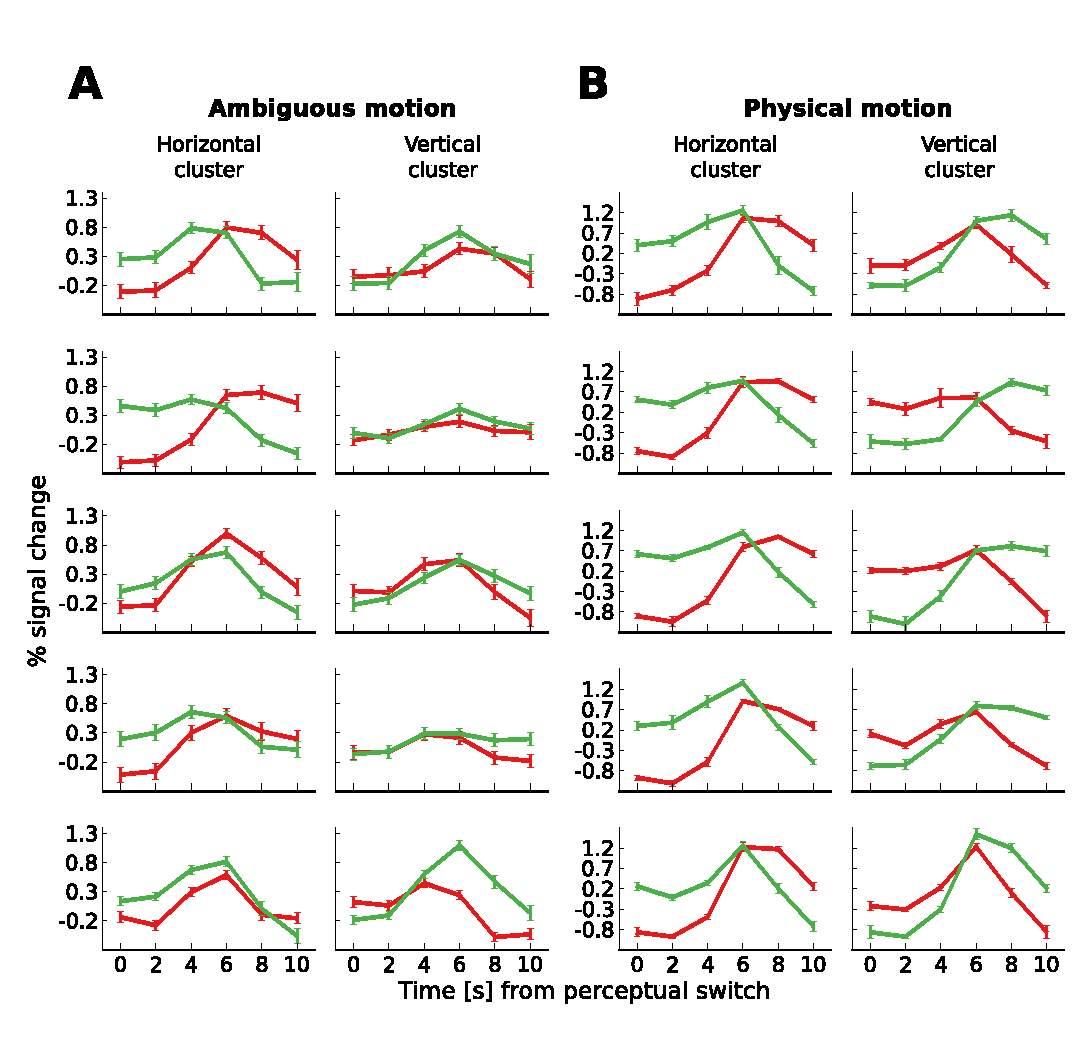
\includegraphics[width=\textwidth]{figures/chapter_03/fig2.eps}
\caption{Single-subject event-related averages for ambiguous and physical motion. \textbf{(A)} Lines show event-related sample means across perceptual periods during ambiguous motion. Error bars represent standard deviation of the mean across perceptual periods. \textbf{(B)} Lines show event-related sample means across cross-validation folds during physical motion. Error bars represent standard deviation of the mean across cross-validation folds. Both panels show responses for either horizontal clusters (on the respective left) or vertical clusters (on the respective right of the panel), separately for every subject (rows). Time courses (normalized to run average) are displayed during horizontal (red lines) and vertical (green lines) perceptual periods. At time point 0s subjects reported a perceptual switch specifying whether they now perceived horizontal or vertical motion.}
\label{fig:single_subject_results}
\end{figure}

To determine to which extent the cluster signals reflected the perceived as opposed to the physical stimulus, we compared signal changes during physical and ambiguous motion. For the physical motion quartet both retinal and perceived motion axis changed, while for the ambiguous motion display only the perceived motion axis changed. Figure ~\ref{fig:single_subject_results}B shows the average fMRI time course for every subject during the physical motion experiment. Comparison of responses during the two experiments revealed a similar qualitative pattern. Quantitatively, the amplitude modulations were larger for physical than for ambiguous motion (Table ~\ref{tab:modulations}).

Upon visual inspection we found voxel preferences between physical and ambiguous motion to be spatially overlapping (Figure ~\ref{fig:consistency}A). Thus, when voxels showed a horizontal preference during physical motion, they often showed the same preference during ambiguous motion. To assess the consistency in preference we computed correlations between preferences during the two experiments and found significant, positive correlations (Figure ~\ref{fig:consistency}B) in all subjects (S1: r=0.25, p\textless.001; S3: r=0.27, p\textless.001; S7: r=0.27, p\textless.001; S8: r=0.21, p\textless.001; S9: r=0.22, p\textless.001; two-sided test). This consistency often stayed stable even when we varied the number of voxels included in our region of interest over a larger range (Figure ~\ref{fig:fig3C_supp}).

\begin{figure}[htb!]
\centering
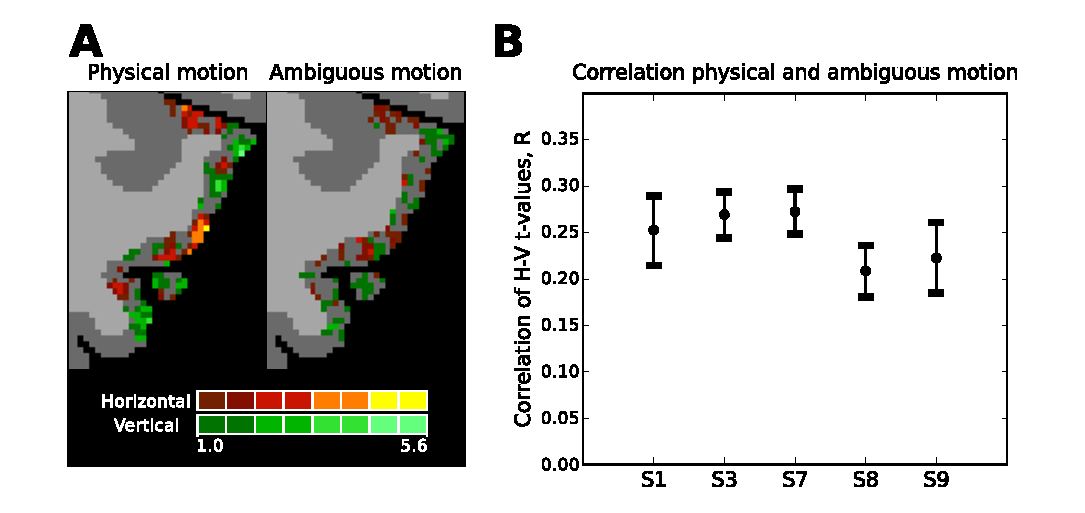
\includegraphics[width=\textwidth]{figures/chapter_03/fig3.eps}
\caption{Consistency of preferences between physical and ambiguous motion. \textbf{(A)} Qualitative consistency. Preferences for either horizontal (red) or vertical (green) motion are shown on the transverse slice of a selected subject (S1, left area hMT+) during either physical (left) or ambiguous (right) motion. Perceptually brighter colors indicate a higher degree of preference. Preferences are overlaid on segmentation labels of white (white-gray voxels) and gray matter (dark-gray voxels). \textbf{(B)} Quantitative consistency. Displayed are the median bootstrapped correlation coefficients for t-values of the contrast horizontal \textgreater vertical found for physical and ambiguous motion. Voxels were selected based on independent data from the hMT+ localizer. Every point represents the result of a single subject (S1, S3, S7, S8, S9). Error bars represent the 2.5th and 97.5th percentile of the bootstrapped correlation coefficients.}
\label{fig:consistency}
\end{figure}

To exclude the possibility that differences in retinotopic preferences are responsible for our observed effects, we conducted several control experiments. First, we showed that the identified clusters display expected axis-of-motion tuning on two independently acquired data sets (Figure  \ref{fig:figI_motionTng}A,B). Second, we estimated the visual field coverage for both horizontal and vertical clusters and did not find a difference in their coverage of the horizontal and vertical motion trajectory (S3: t(205)=0.066, p=.948; S7: t(729)=1.26, p=.209) (Figure ~\ref{fig:figH_retinotopy}). Third, we selected voxels for horizontal and vertical clusters based on horizontal and vertical motion conditions that were retinotopically matched (Figure ~\ref{fig:figI_motionTng}C) and obtained responses in these clusters during ambiguous motion. In 3 out of 3 horizontal clusters (S1: t=4.22, p=.002; S3: t=9.35, p\textgreater.001; S9: t=5.26, p\textgreater.001; 1000-fold permutation) and in 2 out of 3 vertical clusters (S1: t=3.86, p=.048; S3: t=-4.44, p=.018; S9: t=3.44, p=.014; 1000-fold permutation), the amplitude reflected perceived motion axis. This finding was robust to a varying number of voxels included in the clusters (Figure ~\ref{fig:figI_motionTng}D).

Finally, we wondered whether preferences for horizontal and vertical motion showed a form of cortical organization akin to columns selective for a particular motion axis. To address this question, we zoomed in to the observed responses (Figure ~\ref{fig:clusters}A) by constructing regular, high-resolution grids that covered the identified hMT+ areas (Figure ~\ref{fig:clusters}B) \parencite{Zimmermann2011,Kemper2017}. The grid allowed us to visualize and quantify how motion preferences change in the direction of cortical depth and along the cortical surface. If motion preferences are organized in a columnar fashion, they should stay stable in the direction of cortical depth and change when moving along the cortical surface. Using Meng's z-test \parencite{Meng1992}, we found that physical motion preferences at corresponding points along the cortical depth were more correlated to each other than preferences at grid points separated by a similar distance along the cortical plane (Figure ~\ref{fig:clusters}C, \ref{fig:fig4F_supp}) \parencite{Nasr2016} in all subjects (S1: z=12.76, p\textless.001; S3: z=11.54, p\textless.001; S7: z=18.11, p\textless.001; S8: z=3.80, p\textless.001; S9: z=8.33, p\textless.001; two-sided test) (Figure ~\ref{fig:clusters}D). A comparison of directional spatial autocorrelation corroborated this finding (Figure ~\ref{fig:figJ_autoCorr}). Preferences during ambiguous motion showed smaller and less consistent correlation differences (S1: z=-3.26, p=.001; S3: z=6.09, p\textless.001; S7: z=3.08, p=.002; S8: z=7.73, p\textless.001; S9: z=-0.21, p=.837; two-sided test).

\begin{figure}[htb!]
\centering
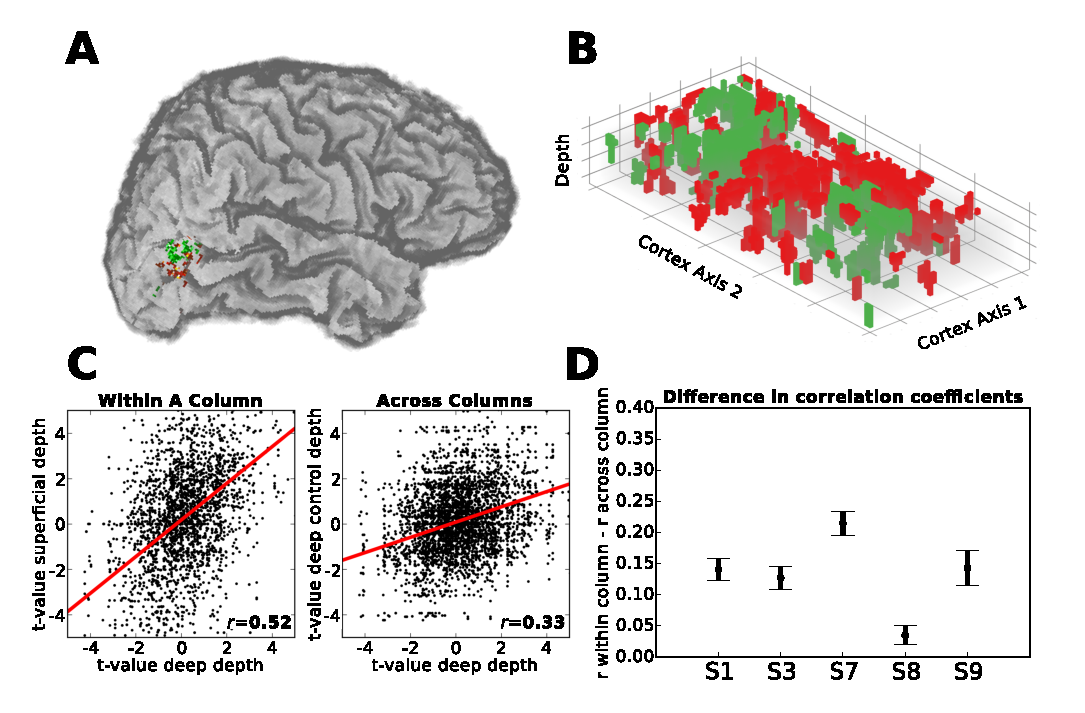
\includegraphics[width=\textwidth]{figures/chapter_03/fig4.eps}
\caption{Horizontal and vertical columnar-like clusters for physical motion. Based on data from the physical motion experiment, voxels were colored in either red (horizontal motion preference) or green (vertical motion preference). \textbf{(A)} Functional hMT+ clusters shown on an individual brain. \textbf{(B)} Functional responses to physical motion were sampled using a regular 3D grid. Cortex axis 1 and 2 represent the cortical plane; the z-axis represents cortical depth. \textbf{(C)} Correlation of axis preference sampled for deep and corresponding superficial depth level (left) or at different nearby locations in deep depth level only. Results are shown for a selected subject and hemisphere (S7, left hemisphere). \textbf{(D)} Subject-wise 95 percent confidence intervals for the difference in z-transformed correlation coefficients within and across grid columns. Every interval represents the result of a single subject (S1, S3, S7, S8, S9). "Col" stands for column.}
\label{fig:clusters}
\end{figure}

\section{Discussion}
Our results support findings of previous human fMRI studies \parencite{Sterzer2002,Muckli2002,Castelo-Branco2002, Kamitani2006, Brouwer2007} that area hMT+ makes up part of the content-specific NCC by demonstrating a link between the experience of visual motion and response amplitudes in area hMT+. Most importantly, our findings extend this idea by demonstrating involvement of specific horizontal and vertical hMT+ clusters in tracking conscious experience of a particular motion axis. Earlier human fMRI studies demonstrated a coupling between categorical contents of consciousness and activity in macroscopic human areas \parencite{Tong1998,Hasson2001,Andrews2002}. In those studies the two competing perceptual states pertained to two different categories (e.g. face vs. building or face vs. object) and experience of these categories was shown to be reflected in the amplitude of different category-specialized areas like FFA or PPA. By contrast, in our study the two perceptual states fell within the same category (motion) and were distinguishable only by subordinate categorical differences (horizontal vs. vertical).

fMRI studies that have compared sub-category perceptual states \parencite{Sterzer2002,Muckli2002,Castelo-Branco2002} were limited by spatial resolution and could only distinguish the states by global amplitude differences of the same area. Although studies using multivariate pattern analysis \parencite{Kamitani2006, Brouwer2007} detected small activation differences between two perceptual states, these studies did not unequivocally reveal the underlying spatial organization of such activation patterns \parencite{Logothetis2008} since the existence of two types of patterns does not imply the existence of two different neural populations \parencite{Bartels2008}. Problematically, this complicates interpretation since coarse-scale biases might account for found differences \parencite{Wang2014}. In comparison, using sub-millimeter resolution, our study could link sub-category contents of consciousness to dissociative amplitude modulations in distinct populations within the same brain area.

Several studies indicate that not all signals that modulate with a reported conscious state reflect the conscious experience itself. Instead, at least in part, these signals reflect processes that precede or follow the experience, among them monitoring the experimental task, planning and reporting \parencite{Koch2016,DeGraaf2012,Frassle2014}. Although we cannot exclude the possibility that some of the response modulation we observed resulted from button presses to report the perceived axis of motion, this interpretation is not in line with findings that activity for reporting and task monitoring is localized to frontal, executive areas, and not to occipital visual cortex \parencite{Frassle2014}. Furthermore, button presses were counterbalanced across the two scanning sessions, making it unlikely that they caused the observed response modulations, which by design needed to be consistent across sessions.

The signal modulations that we found to reflect the conscious percept were based on average cluster responses. It is therefore possible that, although as a whole the cluster showed modulation in the expected direction, a subgroup of voxels did not (or only to a lesser degree) modulate its signal with the percept. Indeed, when we compared amplitude modulations for ambiguous and physical motion (Figure ~\ref{fig:single_subject_results}, Table ~\ref{tab:modulations}), we found larger modulations in response to the latter. One explanation for this difference is that the physical motion stimulus gives rise to both physical bottom-up and perceptual lateral and top-down processes, while the ambiguous motion display invokes primarily perceptual lateral and top-down processes. Earlier electro-physiology findings that only about 40\% of identified MT neurons modulated their spiking with the dominant motion direction in binocular rivalry \parencite{Logothetis1989} are in line with this interpretation. One idea inspired by animal physiology \parencite{Felleman1991, Markov2014} is that bottom-up and lateral / top-down processes recruit different laminar parts of a column. This idea could account for our observation that preferences during ambiguous motion displayed less consistent columnarity than during physical motion. To fully illuminate this possibility, one would need to distinguish the specific laminar contributions to activity in a column, which is beyond the scope of this chapter and subject to future studies.

Our study follows recent advances in ultra-high field MRI which now allow for probing functional responses at the level of mesoscopic structures such as columns and layers \parencite{Polimeni2017, DeMartino2016, Kemper2017}. Previous studies have identified columnar-like structures in humans in V1 \parencite{Cheng2001, Yacoub2008}, V2 and V3 \parencite{Nasr2016}, V3a \parencite{Goncalves2015} and hMT \parencite{Zimmermann2011}. Yet these studies did not use stimuli that allowed for dissociating neural signals pertaining to conscious perception from those related to sensory stimulation. Using a multistable stimulus, our study indicates that response modulations in columnar structures relate to sub-category contents of consciousness.

The concept of a cortical column has been subject to substantial debate, starting with the first discovery of columns in primary somatosensory cortex of cats \parencite{Mountcastle1956}, and its functional significance has been doubted (see General Discussion). Problematically, the term is used in different ways and as a result the various types of columns that have been identified differ in their defining feature (function, cell constellation, connectivity or myelin content), their extent, and spatial organization \parencite{Rakic2008}. Here, we have used an operational definition of columnarity, where functional preferences were required to be more stable along the vertical than the horizontal extent of cortex. To highlight the difference with microcolumns, which would be beyond the available resolution of current fMRI, or idealized hypercolumns, we have used the term columnar clusters instead of columns throughout.

An alternative explanation of our findings would be that the identified clusters do not reflect a preference for motion axis but for the retinotopic location of the two illusory motion paths. However, our control experiments showed (i) that the selected clusters display characteristic tuning to either the horizontal or vertical motion axis, (ii) that there is no evidence for a difference in population receptive field coverage of horizontal and vertical motion paths and (iii) that even if voxels are selected based on a stimulus with two retinotopically identical conditions only distinguished by motion axis, we still observe modulations with the conscious percept. We believe that, taken together, the results rule out this alternative explanation.

Based on our findings, we suggest that the hMT+ clusters identified here constitute part of the content-specific anatomical neural correlate for experiencing motion axis. Future studies could examine whether similar, clustered organizations exist for sub-category contents of consciousness other than motion axis. The activity in many cortical areas has been shown to be linked to general stimulus categories, including orientations, body parts, houses, faces, words, bigrams and letters. Some of these cortical areas are also known to display columnar organization \parencite{Tanaka2003}. Such research would clarify how the activity of these known functional subunits relates to phenomenal distinctions in conscious content. Furthermore, we pave the way for studies to investigate if columnar clusters represent subordinate dimensions in other high-level phenomena like attention and memory.

\clearpage
\section{Supplementary material}

\subsection{Behavioral results}
All participants reported regular perceptual switches between horizontal and vertical percepts during the ambiguous motion experiment. Across all participants, mean perceptual periods ranged from 7.2s to 13.3s. The average length of horizontal and vertical perceptual periods was 10.8s $\pm$ 1.9s and 10.8s $\pm$ 2.4s (mean $\pm$ standard deviation across subjects), respectively. Goal of the calibration of the motion quartet stimulus during the training session had been 10s long percepts. Figure ~\ref{fig:figF_behRes} shows the average length of horizontal and vertical perceptual periods individually for every subject. For subjects S3 and S9 we found a statistical difference between the length of horizontal and vertical periods (t(249)=-3.78, p\textless.001 and t(336)=4.80, p\textless.001, respectively). For subjects S1, S7 and S8 we found no statistical difference (S1: t(252)=-0.41, p=.685; S7: t(223)=-0.07, p=.947; S8: t(179)=1.14, p=.255). We thus did not observe bias towards one of the two motion axes that was consistent across participants.

\subsection{Results control experiments}
\subsubsection{Control experiment I}
Figure ~\ref{fig:figI_motionTng}A shows the axis-of-motion tuning curves derived from control experiment I in clusters used in the main experiment for two control participants. We observed that clusters showed expected axis-of-motion tuning. Horizontal clusters showed the largest average t-value for the horizontal motion condition, lower t-values for the diagonal motion conditions and the lowest t-value for the vertical motion condition. For vertical clusters we observed a reversed pattern. The permutation testing showed significant correlation for ranks in the horizontal cluster and an idealized horizontally tuned cluster (S1: $\tau$=0.91, p\textless.001; S3: $\tau$=0.91, p\textless.001). Ranks of the vertical cluster correlated significantly with ranks of an idealized vertically tuned cluster (S1: $\tau$=0.91, p\textless.001; S3: $\tau$=0.91, p\textless.001).

\subsubsection{Control experiment II}
Figure ~\ref{fig:figI_motionTng}B shows motion tuning derived from control experiment II for three control participants. All clusters showed tuning in the expected direction such that horizontal clusters show larger average t-values for the horizontal than for the vertical condition and vertical clusters show a reversed pattern. The permutation testing showed significant differences between average t-values for the horizontal and vertical motion condition in both the horizontal (S1: $\bigtriangleup$t=0.43, p\textless.001; S3: $\bigtriangleup$t=0.25, p\textless.001; S9: $\bigtriangleup$t=0.27, p\textless.001) and vertical cluster (S1: $\bigtriangleup$t=-0.65, p\textless.001; S3: $\bigtriangleup$t =-1.21, p\textless.001; S9: $\bigtriangleup$t =-0.68, p\textless.001).

\subsubsection{Control experiment III}
Upon visual inspection, we did not find a difference in visual field coverage between horizontal and vertical clusters (Figure ~\ref{fig:figH_retinotopy}A). All clusters showed coverage of the area between and foveal to the inducer squares. We found that clusters had more coverage of the vertical than the horizontal trajectory (Figure ~\ref{fig:figH_retinotopy}B), which was significant in all clusters (S3 horizontal cluster: t(165)=-4.21, p\textless.001; S3 vertical cluster: t(40)=-6.35, p\textless.001; S7 horizontal cluster: t(522)=-22.15, p\textless.001; S7 vertical cluster: t(207)=-9.40, p\textless.001). This is partially to be expected since the retinotopic trajectory is larger for the vertical than for the horizontal condition (by a factor of 1.26 for both control participants). We did not find a difference between horizontal and vertical clusters in the amount they overlapped with either the horizontal or vertical motion trajectory (S3: t(205)=0.066, p=.948; S7: t(729)=1.26, p=.209). We obtained similar findings when no R2 thresholding was performed and all voxels were included in the analysis (S3: t(549)=-1.56, p=.119; S7: t(1213)=1.40, p=.163).

\subsection{Directional spatial autocorrelation}
Figure ~\ref{fig:figJ_autoCorr} shows how spatial autocorrelation of preferences for physical motion changes with distance both in the cortical depth and the cortical plane direction. Spatial autocorrelation is consistently higher in the cortical depth than in the cortical plane direction, across participants and across a wide range of cortical distances (with the exception of small distances for participant S9). At low cortical distances, the autocorrelation is high both in the cortical depth and plane direction. Autocorrelation decreases with cortical distance for both directions; however, in several participants (S1, S3, S9) remains high in the cortical depth direction even at large cortical distances. Taken together, these observations indicate that motion preferences were more similar in the cortical depth than the cortical plane direction and often remained similar over large cortical distances in the cortical depth direction.

\beginsupplement

\clearpage
\subsection{Supplementary figures}

\begin{figure}[htbp!]
\centering
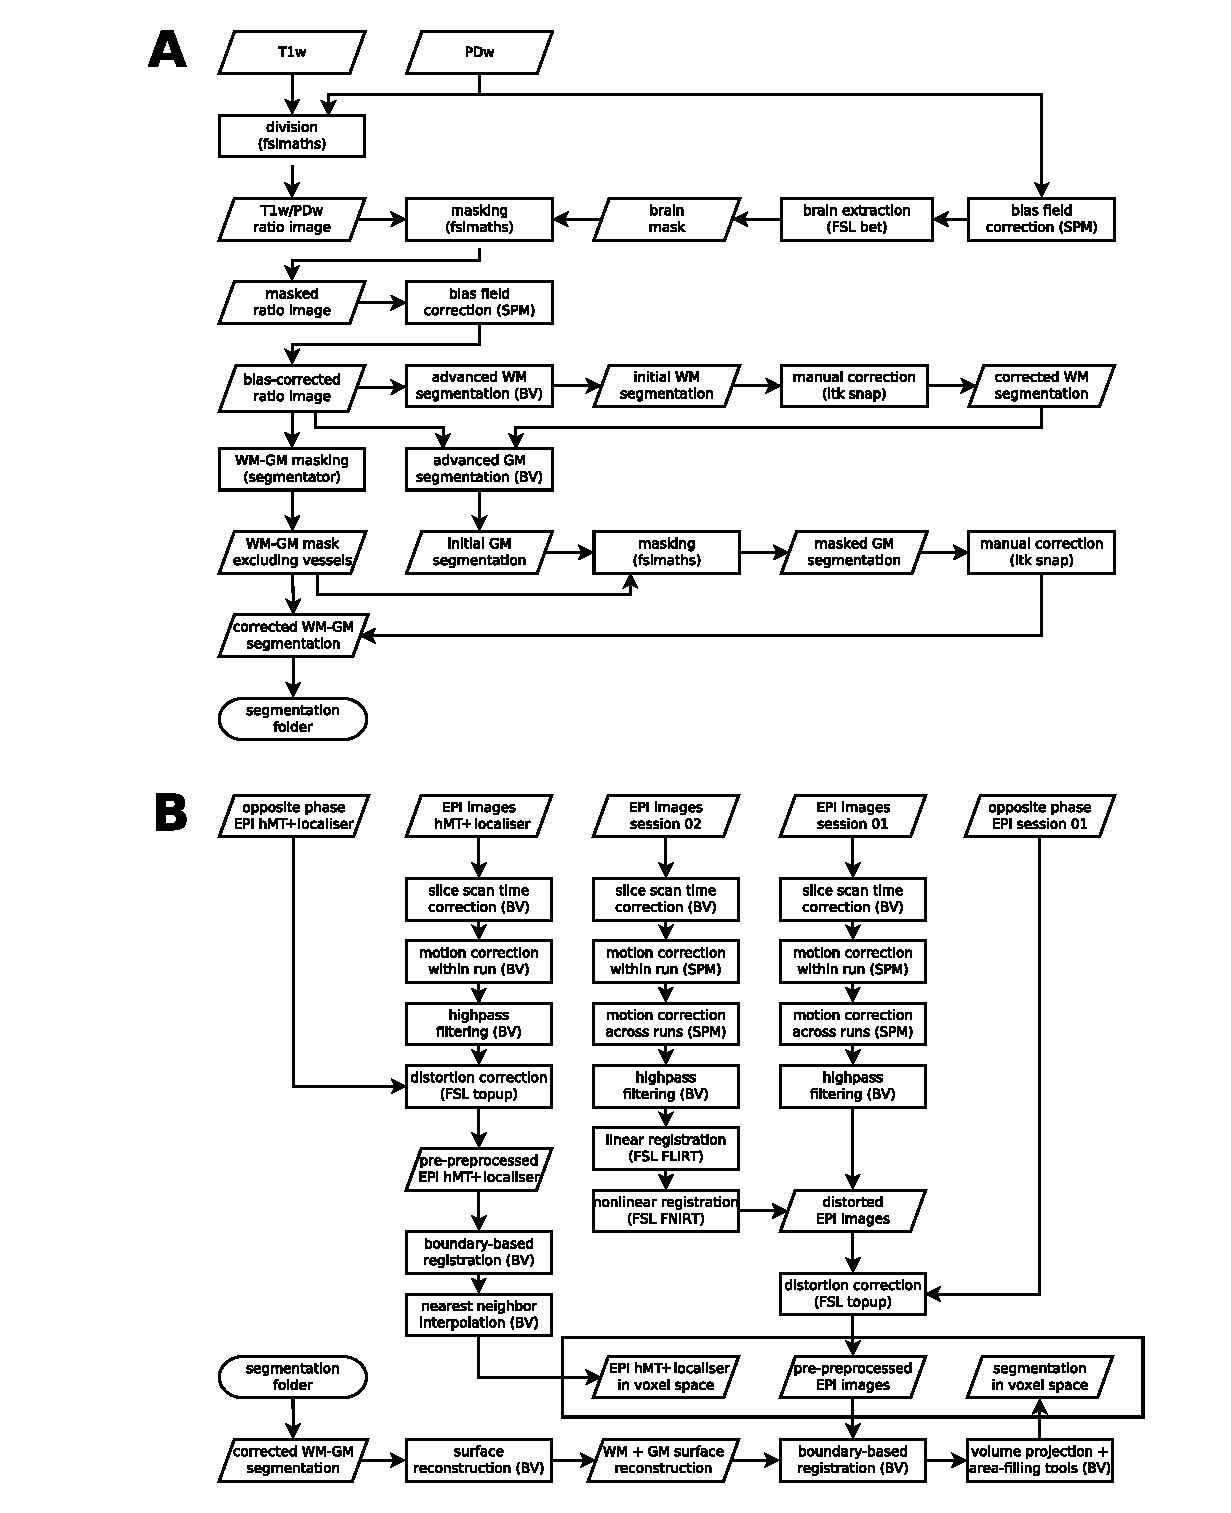
\includegraphics[width=\textwidth]{figures/chapter_03_SI/figS11.eps}
\caption{Overview of pre-processing pipeline. \textbf{(A)} Pre-processing pipeline for structural images. \textbf{(B)} Pre-processing pipeline for functional images. Rectangular shapes represent processing steps, rhombic shapes represent input or outputs and cylindrical shapes represent input or output locations.}
\label{fig:figAB_proc}
\end{figure}

\begin{figure}[htbp!]
\centering
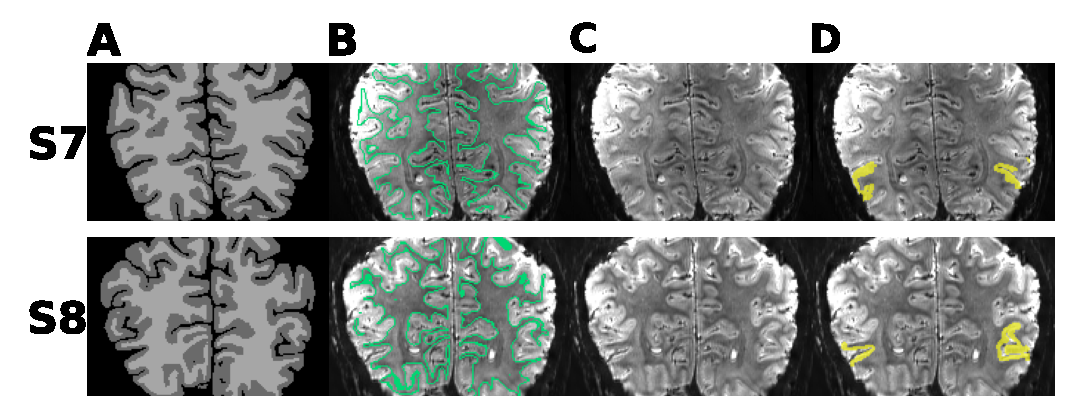
\includegraphics[width=\textwidth]{figures/chapter_03_SI/figS12.eps}
\caption{Segmentation and co-registration quality. All images show coronal slices in radiological convention. \textbf{(A)} Segmentation image showing WM (light gray) and GM (dark gray). Although the segmentation has been down-sampled to the slightly lower resolution of the functional space (0.6 mm isotropic to 0.8 mm isotropic), desirable segmentation features are preserved due to our surface reconstruction pipeline. \textbf{(B)} Overlay of the WM-GM boundary (mint) on the mean functional image in voxel space. High congruence between projected WM-GM boundary (mint) and inherent contrast of functional image (lower intensity values in WM, higher intensities in GM) indicate little segmentation and co-registration error. \textbf{(C)} Mean functional image without segmentation overlay. \textbf{(D)} Mean functional image overlaid with ROI (yellow).}
\label{fig:figC_segmQual}
\end{figure}

\begin{figure}[htb!]
\captionsetup{labelformat=empty}
\centering
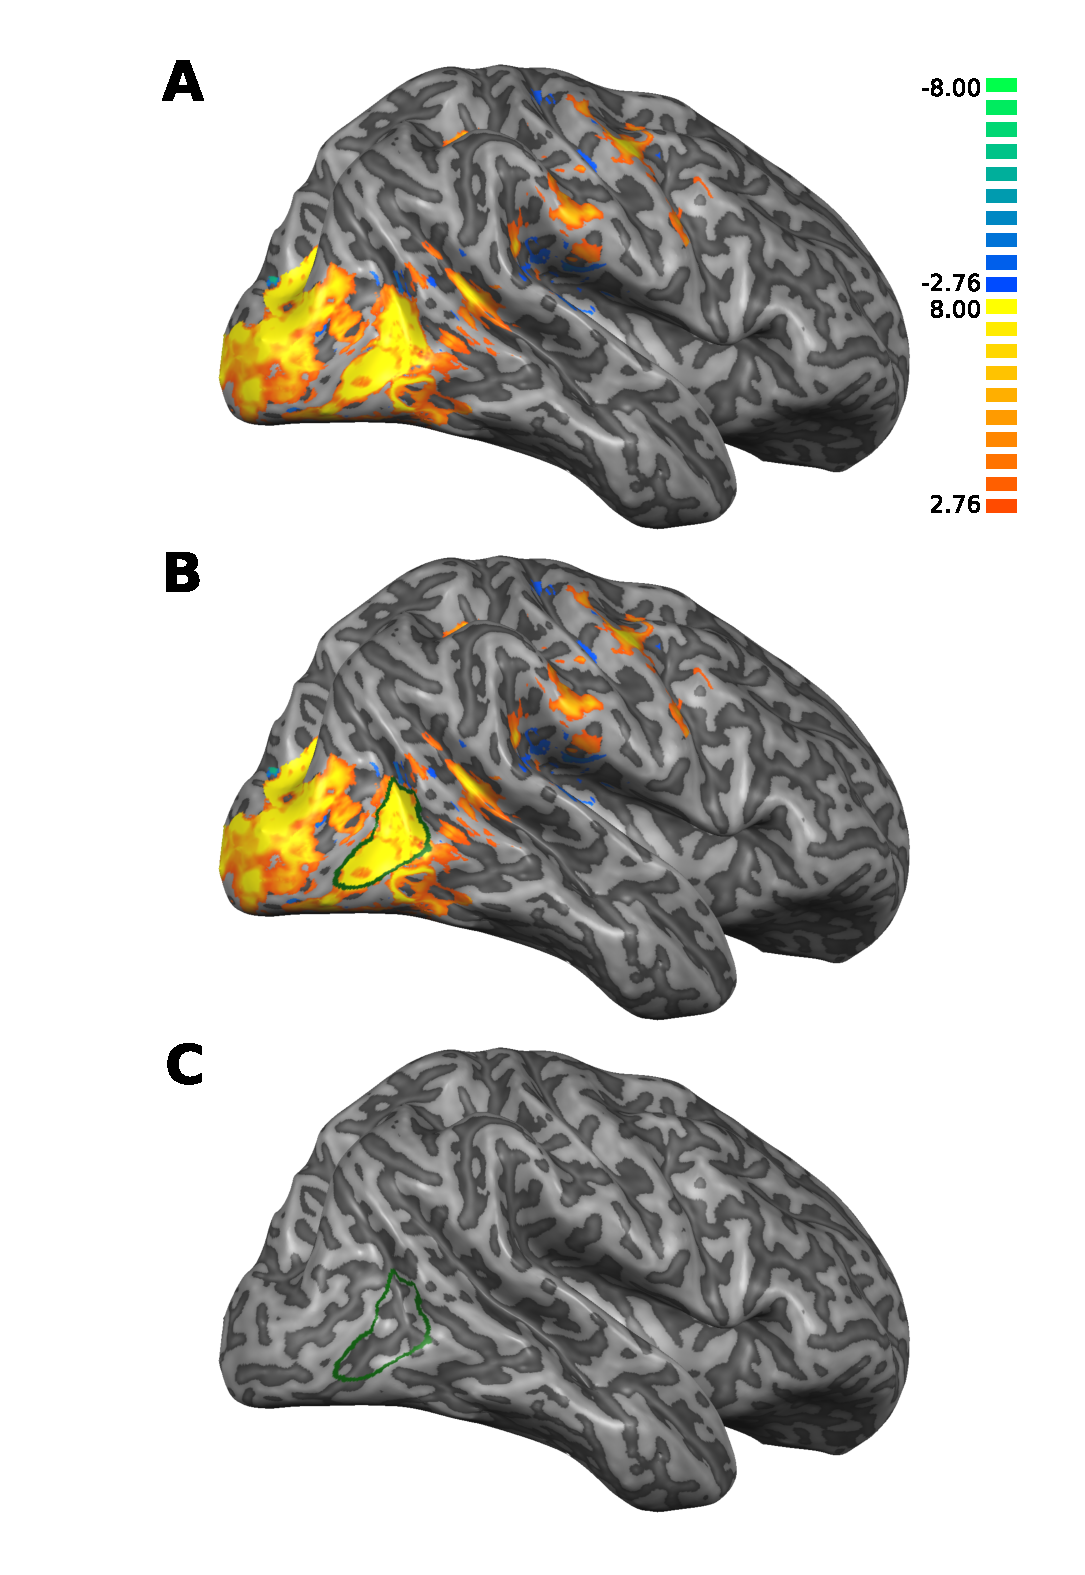
\includegraphics[width=\textwidth]{figures/chapter_03_SI/figS1.eps}
\caption{}
\end{figure}

\begin{figure}[ht!]
\ContinuedFloat
\captionsetup{labelformat=adja-page}
\caption{Example of delineation process for area hMT+. Displayed is the smoothed and inflated right hemisphere of one representative subject (S3). Dark-gray color indicates sulci and light-gray color indicates gyri. \textbf{(A)} Statistical map of responses (t-values) to moving stimuli presented in central apertures (thresholded at q(FDR)\textless.05). \textbf{(B)} Delineation of area hMT+ (green) in the right hemisphere overlaid on top of the statistical map. Selection of area by manual drawing was clearly constrained by the activation map, leaving little room for subjective judgment. \textbf{(C)} Delineation of area hMT+ (green) overlaid without statistical map.}
\label{fig:figD_roiSel}
\noindent\hrulefill
\end{figure}

\begin{figure}[htb!]
\captionsetup{labelformat=empty}
\centering
\includegraphics[width=0.95\textwidth]{figures/chapter_03_SI/figS2.eps}
\caption{}
\end{figure}

\begin{figure}[ht!]
\ContinuedFloat
\captionsetup{labelformat=adja-page}
\caption{Delineations of area hMT+ for all subjects. Displayed are the smoothed and inflated left (left side) and right (right side) hemispheres for all subjects (different rows: S1, S3, S7, S8, S9). Dark-gray color indicates sulci and light-gray color indicates gyri. The delineations of areas hMT+ are overlaid in yellow.}
\label{fig:figE_MtLoc}
\noindent\hrulefill
\end{figure}

\begin{figure}[htb!]
\captionsetup{labelformat=empty}
\centering
\includegraphics[width=\textwidth]{figures/chapter_03_SI/figS3.eps}
\caption{}
\end{figure}

\begin{figure}[ht!]
\ContinuedFloat
\captionsetup{labelformat=adja-page}
\caption{Horizontal and vertical clusters for physical motion. Horizontal (red) and vertical (green) clusters determined by responses during the physical motion experiment are displayed on the smoothed and inflated left (left side) and right (right side) mid-GM reconstructions of area hMT+ for all subjects (different rows: S1, S3, S7, S8, S9). Dark-gray indicates sulci and light-gray indicates gyri.}
\label{fig:figG_clusters}
\noindent\hrulefill
\end{figure}

\begin{figure}[htbp!]
\centering
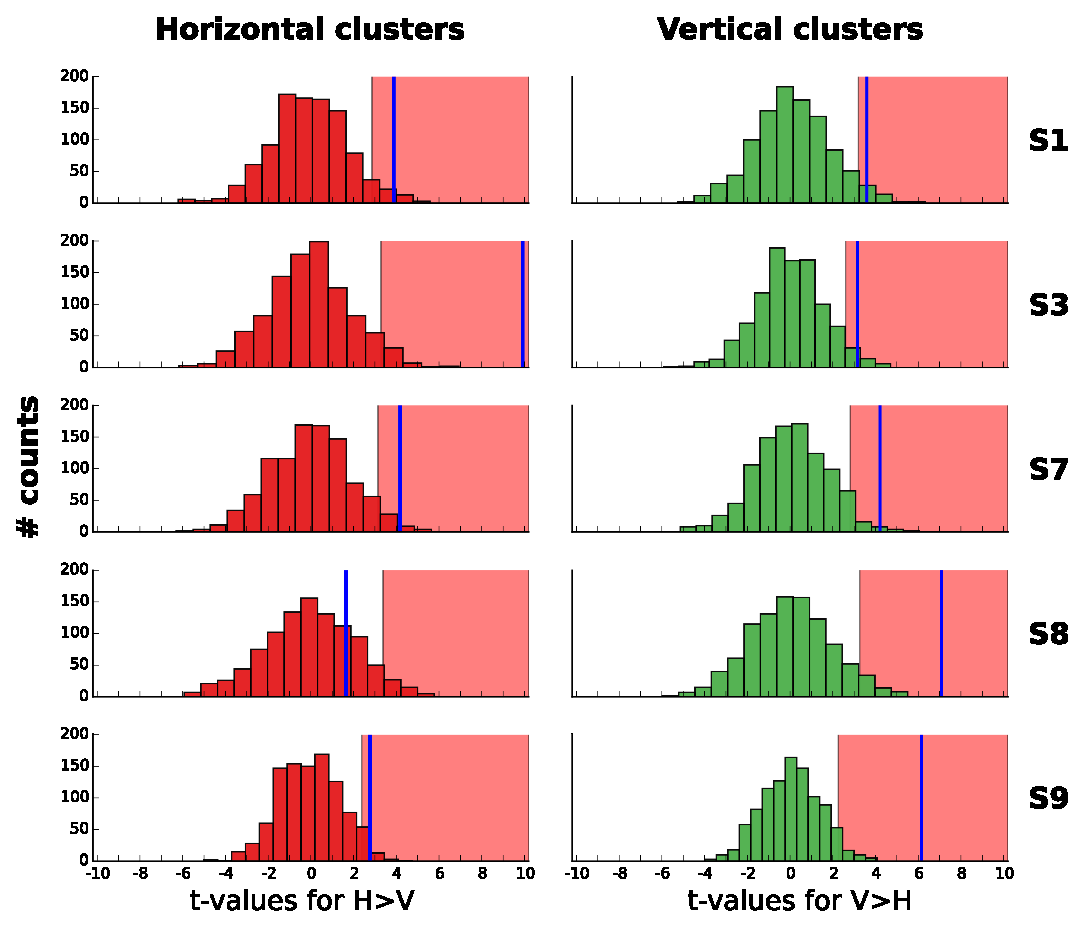
\includegraphics[width=\textwidth]{figures/chapter_03_SI/figS4.eps}
\caption{Results for statistical significance testing of the amplitude modulations during ambiguous motion. The histograms represent a null distribution of t-values obtained by randomly permuting condition labels (1000-fold permutation testing) for either the horizontal (left side, red) or vertical (right side, green) cluster. Blue lines indicate the empirical t-value. Red shading indicates areas above the 97.5th percentile of the null population obtained with 1000-fold permutation testing (rejection area). "H" stands for horizontal, "V" for vertical. Each row represents the results from a different subject.}
\label{fig:fig2C_supp}
\end{figure}

\begin{figure}[htbp!]
\centering
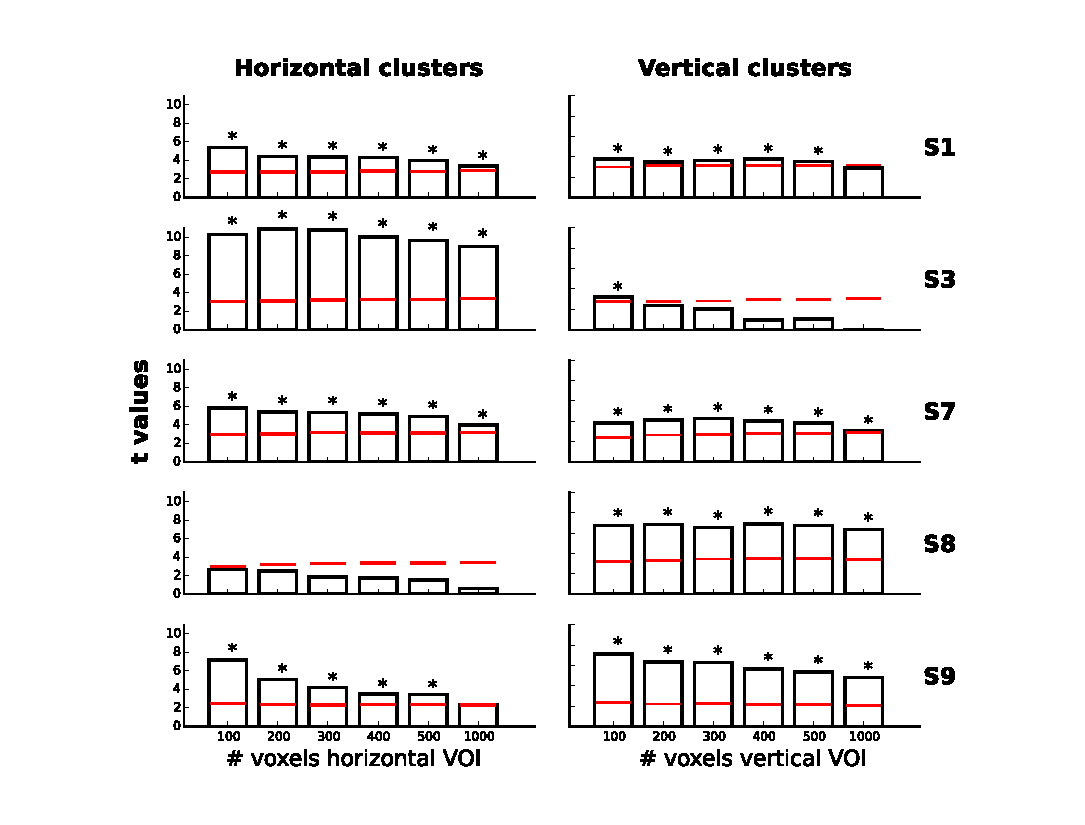
\includegraphics[width=\textwidth]{figures/chapter_03_SI/figS5.eps}
\caption{Observed effects of amplitude modulation during ambiguous motion are robust to changing numbers of voxels included in the ROI. Black bars indicate empirical t-values either for the horizontal (left side) or vertical (right side) cluster. Different bars indicate the results for a particular number of voxels included in the ROI (100, 200, 300, 400, 500, 1000). Red values indicate the 97.5th percentile of a null population obtained with 1000-fold permutation testing. Stars indicate that empirical values fell above the 97.5th percentile of the null distribution. Each row represents the results from a different subject.}
\label{fig:fig2D_supp}
\end{figure}

\begin{figure}[htbp!]
\centering
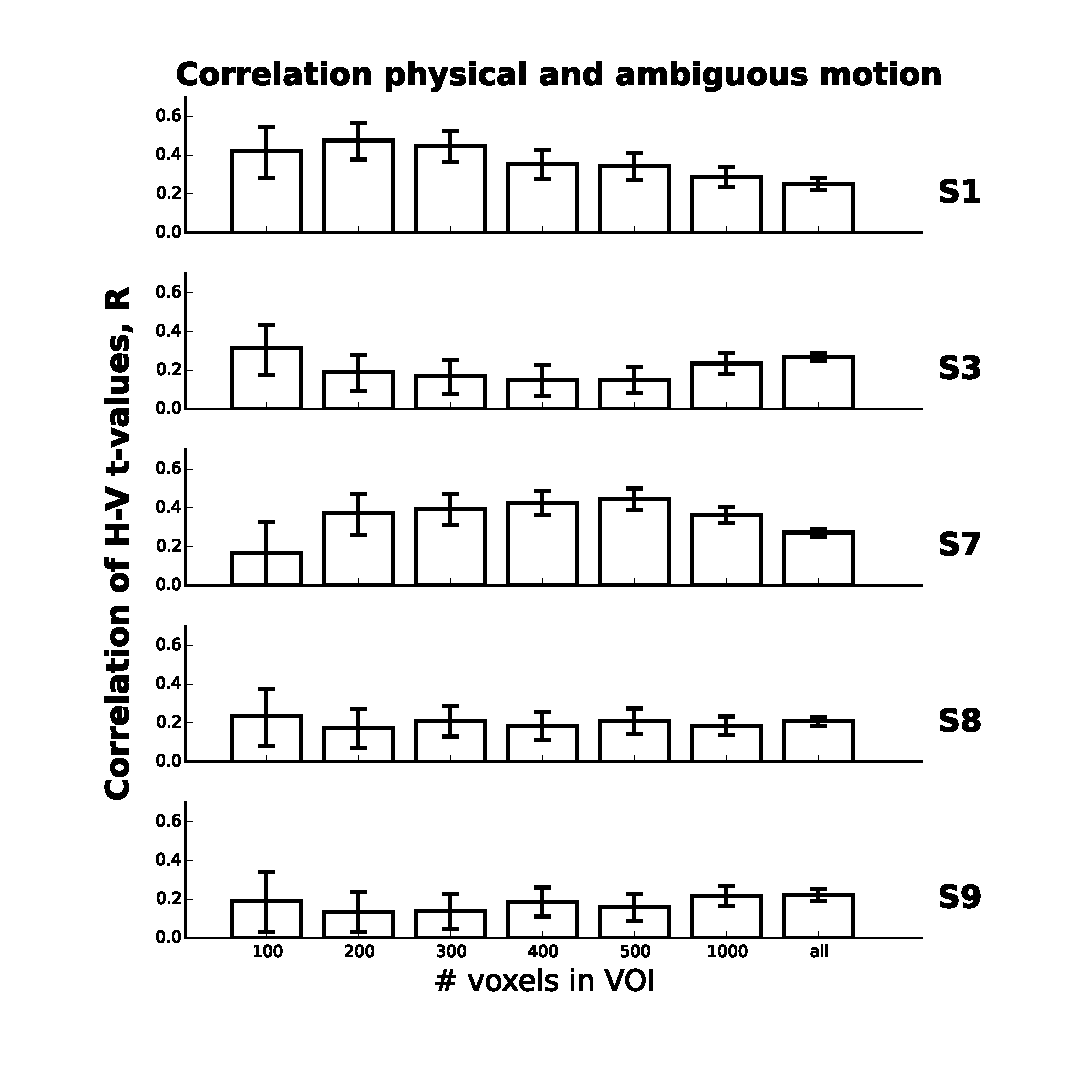
\includegraphics[width=\textwidth]{figures/chapter_03_SI/figS6.eps}
\caption{Consistency in voxel preference was robust to a varying number of voxels included in our ROI. Black bars indicate the median bootstrapped correlation coefficient between t-values for physical and ambiguous motion for a bootstrapped population of voxel values (20,000 re-samples). Error bars represent the 2.5th and 97.5th percentile of the bootstrapped correlation coefficients. Different bars indicate the results for a particular number of voxels included in the ROI (100, 200, 300, 400, 500, 1000). Each row represents the results from a different subject.}
\label{fig:fig3C_supp}
\end{figure}

\begin{figure}[htb!]
\captionsetup{labelformat=empty}
\centering
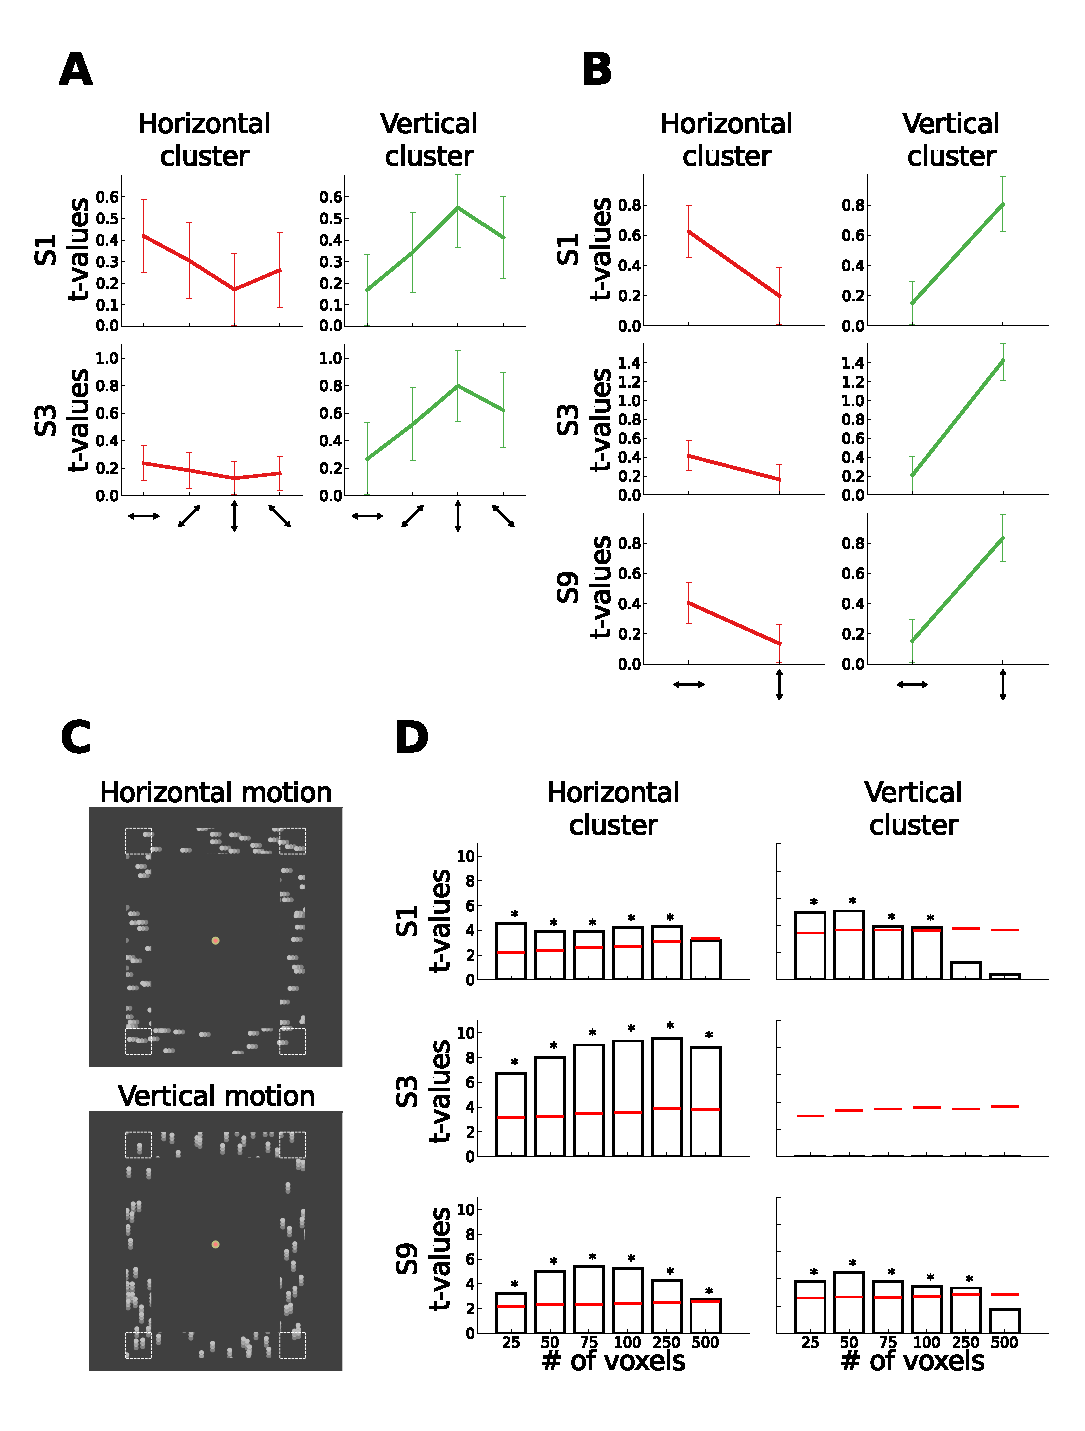
\includegraphics[width=\textwidth]{figures/chapter_03_SI/figS7.eps}
\caption{}
\end{figure}

\begin{figure}[ht!]
\ContinuedFloat
\captionsetup{labelformat=adja-page}
\caption{Clusters show expected motion tuning. \textbf{(A)} Experimental results for control experiment I. Plots show axis-of-motion tuning curves for horizontal (left) and vertical (right) clusters, as used in the main experiment. Lines depict average t-values in response to four presented axes of motion. Error bars represent standard error of the mean. To facilitate visual comparison of tuning curves between clusters, all t-values were normalized such that the lowest response (including its standard error) in a given cluster was equal to zero. This did not change differences between t-values and this step was not performed for data entering statistical analyses. The clusters for the two control participants (S1 and S3, different rows) show expected motion tuning with highest responses to the preferred axis of motion and gradually lower responses to non-preferred axes. \textbf{(C)} Time-lapsed image showing sum of three frames for stimuli used in control experiment II. Retinotopically identical dot fields were moving either horizontally (upper row) or vertically (lower row). Visibility of dots was restricted to the aperture defined by the inducer squares and motion trajectories in the motion quartet experiments. White dashes indicate positions of inducer squares in the motion quartet experiments and were not shown during the actual experiment. \textbf{(B)} Experimental results for control experiment II. Same conventions as for panel \textbf{(A)}, just that in this experiment only horizontal and vertical motion axes were presented and three subjects were recorded (S1, S3 and S9, different rows). Although the underlying data were obtained in independent experiments, the same tuning as in \textbf{(A)} was observed, with highest t-values to the preferred axis of motion. \textbf{(D)} Amplitude modulations during ambiguous motion when data from control experiment II were used to assign voxels to either the horizontal (left) or vertical (right) cluster. Black bars indicate empirical t-values. Different bars indicate results for different numbers of voxels included in the ROI (25, 50, 75, 100, 250, 500). Red bars indicate the 97.5th percentile of a null population obtained with 1000-fold permutation testing. Stars indicate empirical values above the 97.5th percentile of the null distribution. With the exception of one cluster, we can replicate the modulations observed in the main experiment, even though assignment of voxels was based on retinotopically identical conditions.}
\label{fig:figI_motionTng}
\noindent\hrulefill
\end{figure}

\begin{figure}[htb!]
\captionsetup{labelformat=empty}
\centering
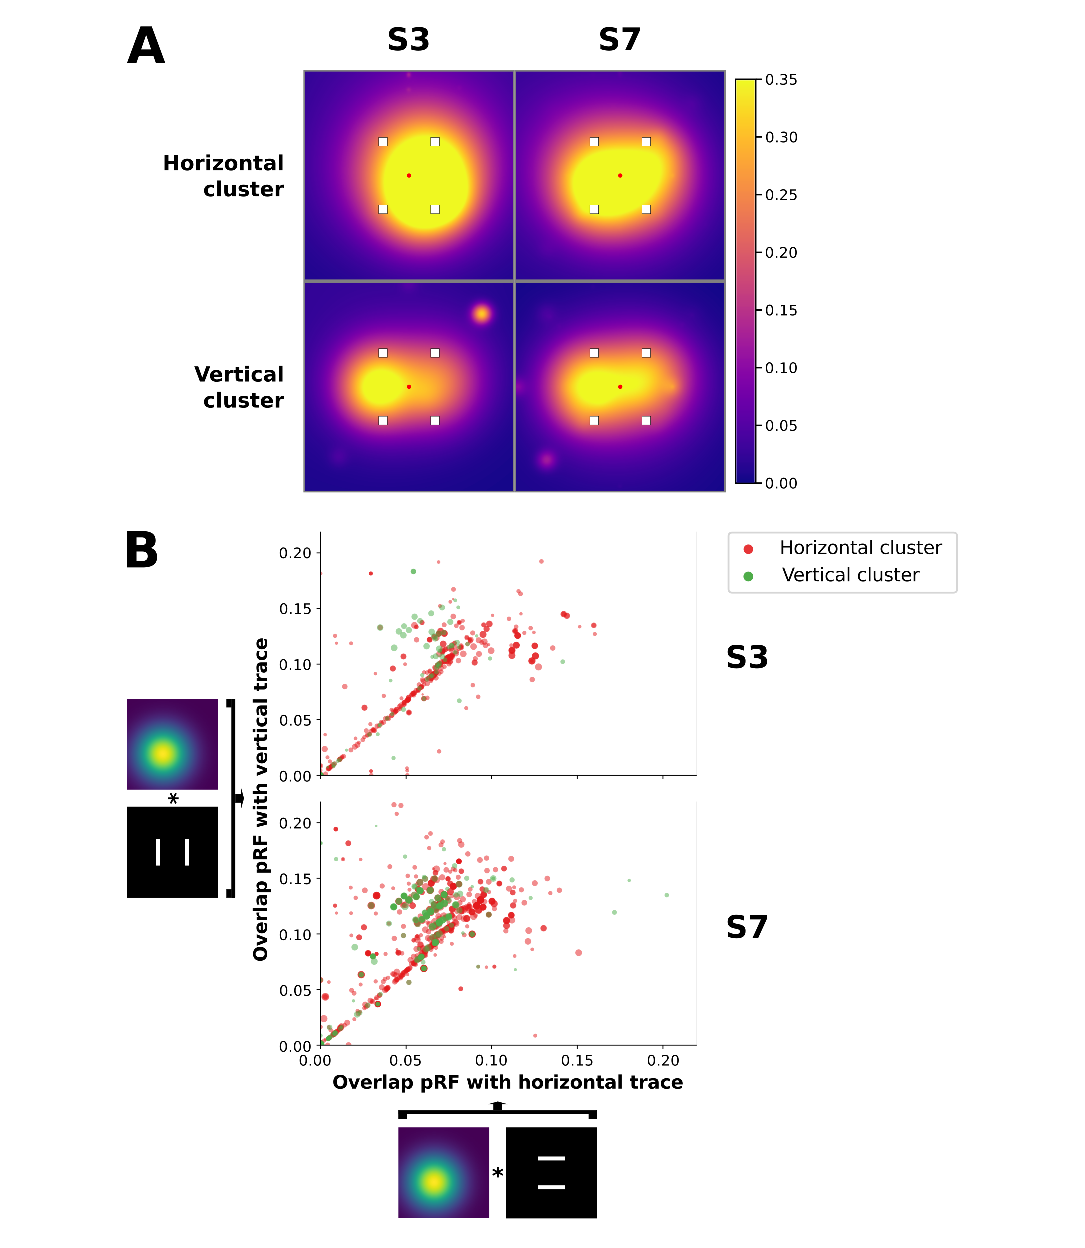
\includegraphics[width=\textwidth]{figures/chapter_03_SI/figS8.eps}
\caption{}
\end{figure}

\begin{figure}[ht!]
\ContinuedFloat
\captionsetup{labelformat=adja-page}
\caption{Clusters show no difference in retinotopic preference. \textbf{(A)} Visual field coverage for either the horizontal (upper row) or vertical (lower row) cluster, as used in the main experiment, for subject S3 (left) and S7 (right). Coverage is computed as the average value across all voxels' population receptive fields (pRF) in a given cluster at every pixel of the visual field (theoretical maximum equal to 1). The subject-specific configuration of the motion quartet is overlaid on top to indicate where inducer squares were presented. Generally, clusters show coverage of the area between inducer squares and foveal to inducer squares. Both horizontal and vertical clusters show a retinotopic bias to vertical motion trajectories but retinotopic bias did not differ between horizontal and vertical clusters. \textbf{(B)} Calculated overlap between the pRF of every voxel in the horizontal (red) and vertical (green) cluster for the horizontal (x-axis) and vertical (y-axis) motion trajectories. Every dot represents a single voxel and dot size is scaled with the fitting accuracy of the pRF model. Results are shown for subject S3 (upper panel) and S7 (lower panel). Many voxels are close to or even on the diagonal, indicating similar or equal overlap with both motion trajectories. The bias towards vertical trajectories observed in \textbf{(A)} is apparent as a cluster of voxels above the diagonal but horizontal and vertical clusters show no difference in this bias.}
\label{fig:figH_retinotopy}
\noindent\hrulefill
\end{figure}

\begin{figure}[htbp!]
\centering
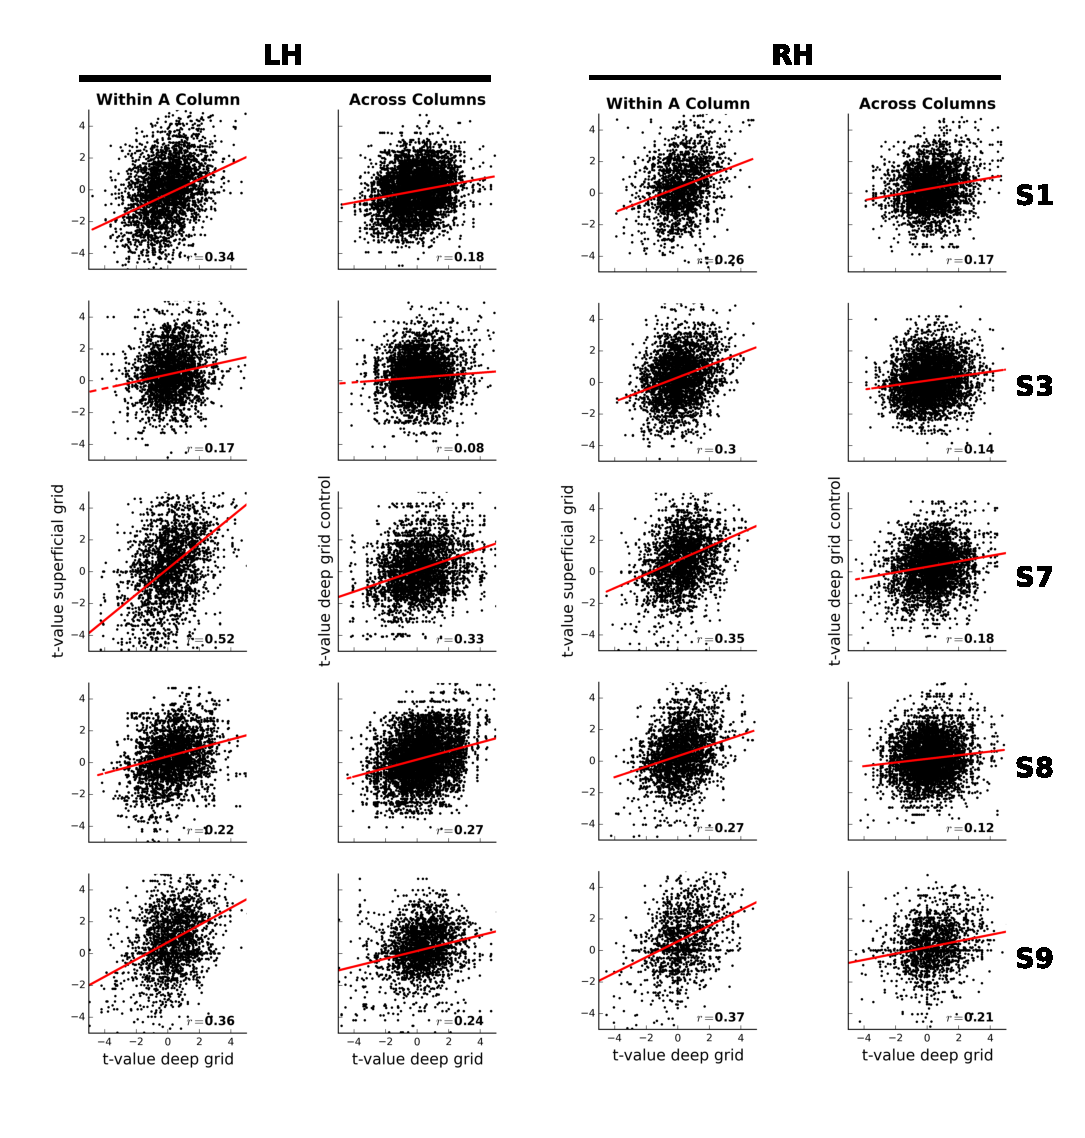
\includegraphics[width=\textwidth]{figures/chapter_03_SI/figS9.eps}
\caption{Motion preferences were more stable in the direction of cortical depth than along the cortical surface. Results are shown for all subjects (rows) and two hemispheres (left hemisphere on the left). Scatter plots show the correlation of axis preference sampled for deep and corresponding superficial depth level ("within a column", respective left side) compared to the correlation for different nearby locations in deep depth level only ("across columns", respective right side).}
\label{fig:fig4F_supp}
\end{figure}

\begin{figure}[htbp!]
\centering
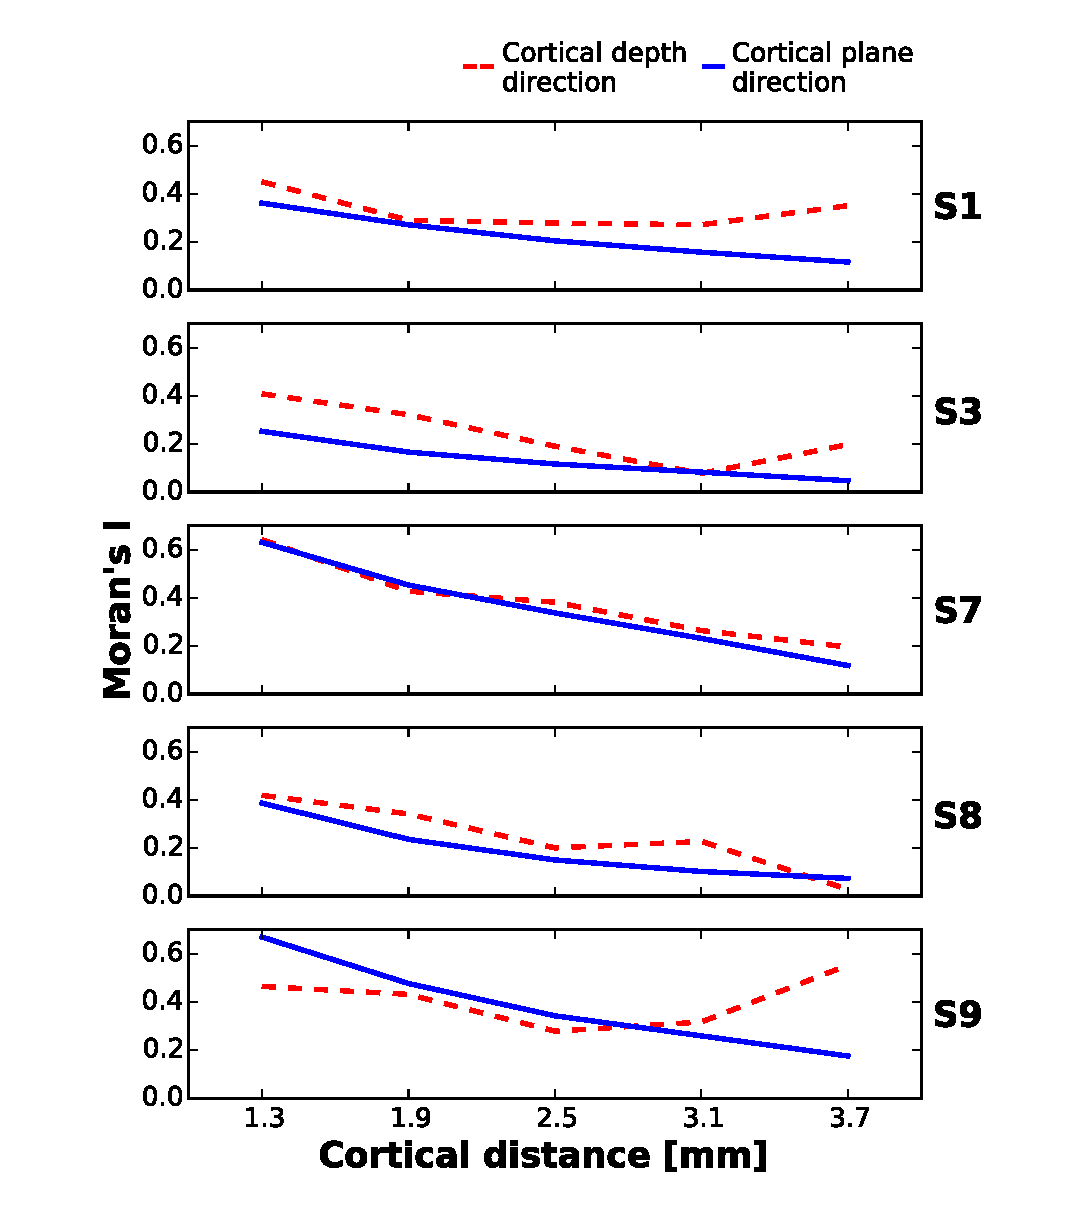
\includegraphics[width=\textwidth]{figures/chapter_03_SI/figS10.eps}
\caption{Greater autocorrelation in cortical depth than in cortical plane direction. Moran's I, a measure of spatial autocorrelation, is plotted over cortical distance (in mm). The red, dashed line shows autocorrelation coefficients in cortical depth (columnar) direction; the blue, solid line shows coefficients in cortical plane direction. Each row shows the results from a different subject.}
\label{fig:figJ_autoCorr}
\end{figure}

\begin{figure}[htbp!]
\centering
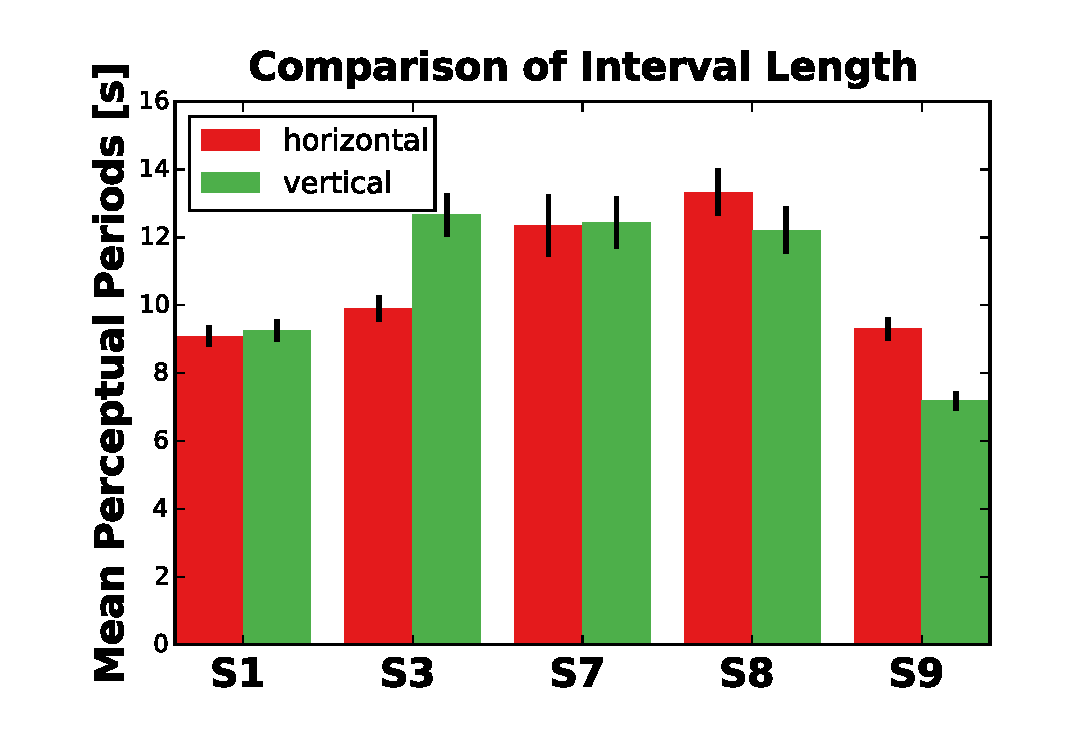
\includegraphics[width=\textwidth]{figures/chapter_03_SI/figS13.eps}
\caption{Average length of perceptual periods. Mean length of perceptual periods in seconds (s) during the ambiguous motion experiment are shown for every analyzed subject (S1, S3, S7, S8, S9), separately for horizontal (red) and vertical (green) perceptual periods. Error bars represent standard error across perceptual periods.}
\label{fig:figF_behRes}
\end{figure}

\clearpage
\subsection{Supplementary tables}

\begin{table}[htbp!]
\centering
\caption{Subject-specific vertical distances for the motion quartet display. Distances are in degrees of visual angle from the fixation point to the center of the square in the motion quartet. Horizontal distance was kept constant at 3 degrees of visual angle.}
\begin{tabular}{cc}
\\
\hline
Subject & Vertical distance \\
\midrule
S1 & 3.8 \\
S3 & 3.9 \\
S7 & 3.9 \\
S8 & 3.9 \\
S9 & 3.8 \\
\bottomrule
\end{tabular}
\label{tab:distances}
\end{table}

\begin{table}[htbp!]
\centering
\caption{Size of the hMT+ ROIs for every subject. LH and RH indicate left and right hemisphere, respectively. Surface area is in square mm.}
\begin{tabular}{cccc}
\\
\hline
Subject & Number of voxels & Surface area LH & Surface area RH
\\
\midrule
S1 & 8341 & 855 & 517\\
S3 & 10267 & 781 & 783\\
S7 & 8394 & 710 & 857\\
S8 & 7923 & 720 & 632\\
S9 & 7361 & 626 & 720\\
\bottomrule
\end{tabular}
\label{tab:rois}
\end{table}

\begin{table}[htbp!]
\centering
\caption{Average cortical thickness of hMT+ ROIs for every subject. LH and RH indicate left and right hemisphere, respectively. 2H means that both hemispheres were included. Std indicates standard deviation.}
\begin{tabular}{cccc}
\\
\hline
Subject & $Mean\pm std$ LH & $Mean\pm std$ RH & $Mean\pm std$ 2H 
\\
\midrule
S1 & $2.74\pm0.55$ &  $2.73\pm0.66$ &  $2.74\pm0.59$\\
S3 & $2.72\pm0.56$ &  $2.84\pm0.65$ &  $2.77\pm0.61$\\
S7 & $2.78\pm0.56$ &  $2.82\pm0.59$ &  $2.80\pm0.57$\\
S8 & $2.58\pm0.53$ &  $2.53\pm0.52$ &  $2.56\pm0.53$\\
S9 & $3.35\pm1.18$ &  $2.47\pm0.46$ &  $2.97\pm1.04$\\
\bottomrule
\end{tabular}
\label{tab:thickness}
\end{table}

\begin{table}[htbp!]
\centering
\caption{Event-related signal modulations during ambiguous and physical motion. Mean trough-to-peak differences $\pm$ standard error of the mean. Positive values indicate that signal increased from the minimum of the first two time points to the maximum of the last two time points. Negative values indicate a signal decrease from the maximum of the first two time points to the minimum of the last two time points. H and V cluster represent the horizontal and vertical clusters defined in the main experiment. H and V percept indicate time periods during which subjects indicated a horizontal or vertical percept. S1, S3, S7, S8 and S9 indicate the different subjects.}
\begin{tabular}{lrllll}
\\
\midrule
\multicolumn{2}{l}{} & \multicolumn{2}{c}{Ambiguous Motion} & \multicolumn{2}{c}{Physical Motion} \\
    &                & H percept      & V Percept      & H percept      & V percept \\
\hline
S1  &                &                &                &                &                \\
    & H cluster      &  1.07$\pm$0.17 & -0.42$\pm$0.26 &  1.92$\pm$0.20 & -1.23$\pm$0.21 \\
    & V cluster      & -0.15$\pm$0.17 &  0.68$\pm$0.22 & -0.50$\pm$0.25 &  1.73$\pm$0.16 \\
\hline
S3  &                &                &                &                &                \\
    & H cluster      & 1.27$\pm$0.16  & -0.89$\pm$0.15 &  1.85$\pm$0.18 & -1.08$\pm$0.16 \\
    & V cluster      & 0.11$\pm$0.15  &  0.30$\pm$0.13 & -0.96$\pm$0.26 &  1.51$\pm$0.21 \\
\hline
S7  &                &                &                &                &                \\
    & H cluster      &  0.89$\pm$0.16 & -0.65$\pm$0.19 &  2.09$\pm$0.12 & -1.23$\pm$0.15 \\
    & V cluster      & -0.37$\pm$0.15 &  0.46$\pm$0.18 & -1.13$\pm$0.19 &  1.91$\pm$0.20 \\
\hline
S8  &                &                &                &                &                \\
    & H cluster      &  0.77$\pm$0.17 & -0.43$\pm$0.18 &  1.82$\pm$0.12 & -0.97$\pm$0.12 \\
    & V cluster      & -0.12$\pm$0.14 &  0.29$\pm$0.20 & -0.79$\pm$0.15 &  1.42$\pm$0.13 \\
\hline
S9  &                &                &                &                &                \\
    & H cluster      &  0.24$\pm$0.13 & -0.75$\pm$0.16 &  2.11$\pm$0.13 & -0.98$\pm$0.13 \\
    & V cluster      & -0.53$\pm$0.14 &  0.79$\pm$0.16 & -0.66$\pm$0.15 &  2.14$\pm$0.12 \\
\bottomrule
\end{tabular}
\label{tab:modulations}
\end{table}

\clearpage
\section{Acknowledgments}
We would like to thank Ingo Marquardt, Faruk Gulban, Sriranga Kashyap, Agustin Lage and Nikolaus Weiskopf for valuable advice.

\stopsupplement
\clearpage
\printbibliography[heading=subbibnumbered, title={References}]